\documentclass[a4paper,twoside]{report}
\input{preamble}
\begin{document}

  \author{Christian Stigen Larsen}
  \date{Draft version: \today}
  \title{Efficient Paxos primitives on a programmable software-defined
    network switch\\\textsf{** DRAFT **}}

  % \frontmatter % <-- Only for book document class
  \maketitle

  \listoftodos % TODO: Remove when finished
  \listoftables
  \listoffigures
  \listofalgorithms
  \lstlistoflistings

  \tableofcontents

  % Should be after ToC, according to University rules
  \chapter{Acronyms}
\begin{acronym}
\acro{SDN}{Software--defined networking}
\acro{TCP}{Transmission control protocol}
\acro{UDP}{Uniform Datagram Protocol}
\end{acronym}


  %\ mainmatter % <-- Only for book document class
  \chapter{Introduction}

\todo{Finn ut rekkefølge på kapittel, feks om bibliography skal være etter appendix}
\todo{Oppdater index til slutt, skriv intro om til slutt, skal vi ha
abstract? legg også til front og back matter, acknowledgments osv}
\todo{Endre tittel til slutt så den er korrekt ifht innhold}

\textbf{\acf{SDN}} \cite{Casado:2005:VNS:1047344.1047383} emerged from
research at Berkeley and Stanford around 2008 as a way to enable networks to
be defined and managed using software
One model of \acs{SDN} is \textit{OpenFlow}\todo{Cite!}, which decouples the control
plane from the forwarding plane in a switch, moving it out to an external
networking node.  It enables one to implement the controller in software.

Although invented quite recently, software-defined networking is already
being heavily used both in academia and industry.  Google, for instance, are
using OpenFlow to ease deploymend and increase utilization in their backbone
networks \cite{crabbe2012sdn} and Stanford has deployed several
OpenFlow-controlled networks on their university network.

In March 2013, IDC \todo{finn ut hva det står for} projected that the SDN market would
  reach \${}3.7 billion by 2016, capturing a 35\%{} share of the switching
  market \cite{Kirkpatrick:2013:SN:2500468.2500473}.
\todo{Skriv om denne setningen, den er tatt nesten direkte fra artikkelen!}

OpenFlow is detailed in chapter \ref{chapter:background.openflow}
\vpageref{chapter:background.openflow}.

\textbf{Paxos}\index{Paxos} \cite{Lamport:1998:PP:279227.279229} is a
family of distributed, fault-tolerant consensus algorithms.  It allows
network nodes to reach \textit{agreement} even in the face of intermittent
network failures.  For example, one can design a database system using Paxos
to make sure that transactions are executed in the same order on all nodes.

Originally published by Leslie Lamport\index{Lamport, Leslie} in 1989, Paxos
has spawned numerous extensions like Byzantine tolerance and so on.  It is
discussed in chapter \ref{chapter:background.paxos} \vpageref{chapter:background.paxos}.

\textbf{Our aim} is to build an efficient, \textit{Paxos-enabled software defined
network}.  Paxos will be implemented on OpenFlow switches to guarantee that
packets sent to all of their connected nodes are sent in the same order.
These end-hosts can run any networking service and leverage the benefits of
Paxos without needing to handle any details of the algorithm.

\section{Hypothesis}

For simplicity, we will constrain our scope to a few primitives of
non-Byzantine, classic crash Paxos in \textit{phase two}, where we have
steady-state flow with no failures.

Furthermore, we want to look at opportunities for increasing networking
performance by moving parts of the Paxos from the control plane down to the
switches' forwarding plane.

We will implement this in progressive stages:

\begin{enumerate}
\item Implement Paxos entirely on an OpenFlow software controller.
\item Extend OpenFlow and Open vSwitch so we can transfer bytecode down to
the software switches.
\item Move parts of the Paxos implementation down to the forwarding plane
(OpenFlow \textit{flow tables}), achieving a good balance of performance and
programming maintainability
\end{enumerate}

Our hypothesis is two-fold:

\begin{enumerate}
\item Network nodes can leverage Paxos guarantees \textit{transparently} by
implementing it on the software switches using OpenFlow.
\item We can achieve good relative performance by moving parts of the
implementation from the OpenFlow controllers down to the software switches.
\end{enumerate}

We aim to build a proof-of-concept sytem backing up these claims.  The
thesis will therefore be a study of \textit{feasibility}.

\section{Overview}

\todo{FLytt dette inn i teksten over, trenger ikke være egen section.}
We discuss the theoretical background needed to understand this thesis in
chapter \ref{chapter:background} \vpageref{chapter:background}.  If you already know \acs{SDN},
OpenFlow and Paxos, you can skip this chapter.

Then we look at what OpenFlow can offer us in chapter
\ref{chapter:details.openflow}
\vpageref{chapter:details.openflow}, detail what Paxos requires for
implementation in chapter \ref{chapter:details.simplified.paxos} 
\vpageref{chapter:details.simplified.paxos} and propose a
design based on this in chapter \ref{chapter:design} \vpageref{chapter:design}.
\todo{Sjekk at linker stemmer, kan gjerne forenkles også + forbedres}

Finally, we .... blabla ... look at benchmarks and conclude in chapter
\ref{chapter:conclusion} \vpageref{chapter:conclusion}.

\section{Scope}

\todo{Skriv mere og bedre}

We will only look at a simplified version of Paxos in which we only
implement accept and learn messages. We ignore liveness checking such as
heartbeats. We ignore implementing the expanded OpenFlow features in the
network protocol and controller. We only look at steady state Paxos.
We assume switches are colocated. etc etc etc.

We also ignore the fact that if a switch goes down and back up again, it
will need to rejoin the Paxos network and its end-hosts need to synchronize
state (or just copy the state from a host on another switch).

\section{Topology}

\todo{Kan kanskje flyttes opp til hypothesis? Vis først HVA vi vil gjøre, og
  så hypotese}

Here we present what we want to achieve.  First, let's look at the situation
for one switch.

\begin{figure}[H]
  \centering
  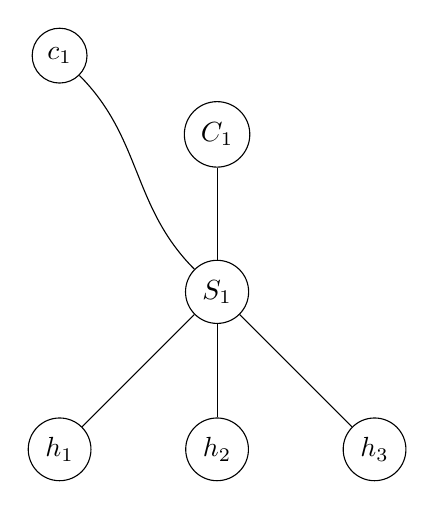
\begin{tikzpicture}[every node/.style={draw, circle}]
    \node (c1)    at (-2,  3) {$c_1$};
    \node (ctrl1) at ( 0,  2) {$C_1$};
    \node (S1)    at ( 0,  0) {$S_1$};
    \node (h1)    at (-2, -2) {$h_1$};
    \node (h2)    at ( 0, -2) {$h_2$};
    \node (h3)    at ( 2, -2) {$h_3$};

    \draw (c1) to[out=315,in=135] (S1);
    \draw (S1) -- (ctrl1);
    \draw (S1) -- (h1);
    \draw (S1) -- (h2);
    \draw (S1) -- (h3);

  \end{tikzpicture}
  \caption{A single switch $S_1$ with its controller $C_1$, end-hosts
    $h_1, h_2, h_3$ and one WAN-side client $c_1$.}
  \label{figure:graph.single.switch}
\end{figure}

For an explanation of our nomenclature, we will always talk about
\textit{clients} as being remote hosts on the \ac{WAN} side.

The clients are supposed to be placed on the \ac{WAN}---but they are actually
just ordinary hosts on each switch.  We just \textit{pretend} they are
placed on the WAN.  It really doesn't matter, though, as all of their
communication goes through each respective switch.

The \textit{end-hosts} are nodes connected to a single switch and running
services such as key-value stores, lock servers, logging servers,
databases, and so on.

Here is the situation with three switches---the minimum number nodes we need
in a Paxos system.  We have added all-to-all links between the switches in
case any one of them should go down.

\begin{figure}[H]
  \centering
  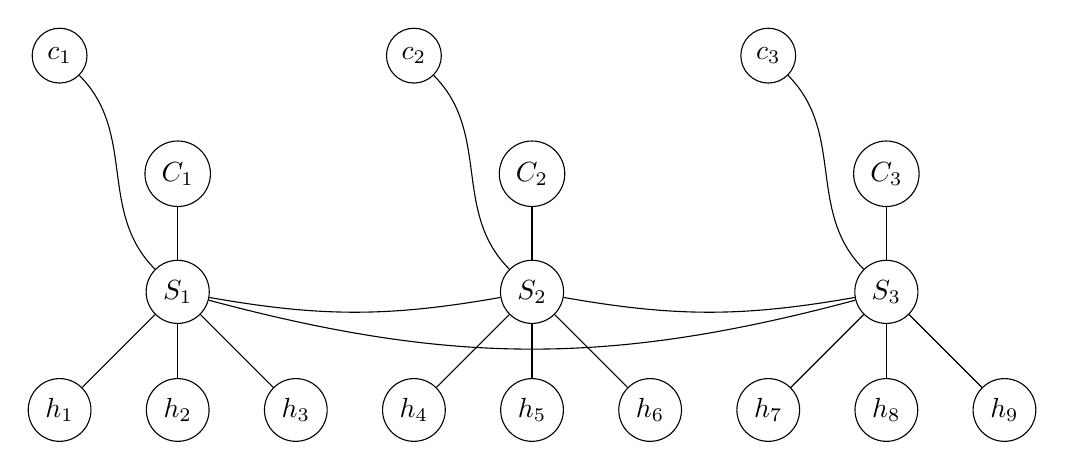
\begin{tikzpicture}[every node/.style={draw, circle},x=0.75cm,y=0.75cm]
    \foreach \n in {1,2,3} {
      \pgfmathsetmacro\x{(\n-2)*6}
      \node (c\n)    at (\x - 2,  4) {$c_\n$};
      \node (ctrl\n) at (\x ,  2) {$C_\n$};
      \node (S\n)    at (\x ,  0) {$S_\n$};

      \draw (c\n) to[out=315,in=135] (S\n);
      \draw (S\n) -- (ctrl\n);

      \foreach \h in {1,2,3} {
        \pgfmathsetmacro\pos{(\h - 2)*2}
        \pgfmathtruncatemacro\num{((\n - 1)*3) + int(\h)}
        \node (h\num) at (\x + \pos, -2) {$h_{\num}$};
        \draw (S\n) -- (h\num);
      }

    }

    % Links between switches
    \draw (S1) to[out=-10,in=190] (S2);
    \draw (S2) to[out=-10,in=190] (S3);
    \draw (S1) to[out=-15,in=195] (S3);

  \end{tikzpicture}
  \caption{Three switches $S_1, S_2, S_3$ with controllers $C_1, C_2, C_3$ acting as Paxos nodes.}
  \label{figure:graph.three.switches}
\end{figure}

The point is that these services will be mirrored by the use of our
Paxos-enabled switches.  For our purposes, we will assume that the services
on these hosts are \textit{deterministic}\footnote{Or, more correctly,
\textit{referentially transparent}.} in the sense that the parameters
uniquely determine the state of the service after being processed---if two
hosts running the same service receive the exact same packet, their state
will be identical after having processed it.  This is a prerequisite for our
system.  The OpenFlow switches, running Paxos, will only make sure that
packets are delivered in the \textit{same order} to the end-hosts.

\section{Viability}

Why would such a system be useful? Consider the situation of implementing
Paxos in code on some servers, running services such as key-value stores,
etc.

\begin{figure}[H]
  \centering
  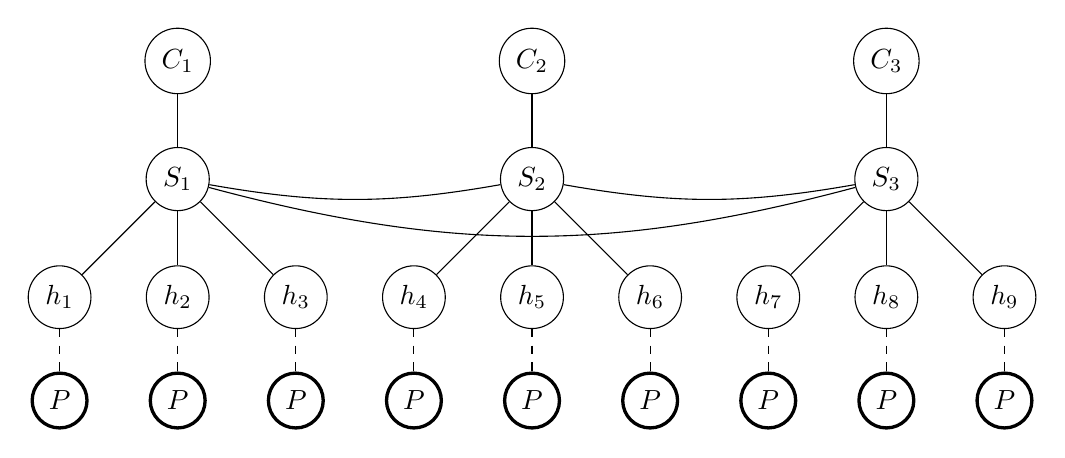
\begin{tikzpicture}[every node/.style={draw, circle},x=0.75cm,y=0.75cm]

    % For each switch ...
    \foreach \n in {1,2,3} {
      \pgfmathsetmacro\x{(\n-2)*6}
      \node (ctrl\n) at (\x ,  2) {$C_\n$};
      \node (S\n)    at (\x ,  0) {$S_\n$};

      \draw (S\n) -- (ctrl\n);

      % For each host ...
      \foreach \h in {1,2,3} {
        \pgfmathsetmacro\pos{(\h - 2)*2}
        \pgfmathtruncatemacro\num{((\n - 1)*3) + int(\h)}

        % Host node
        \node (h\num) at (\x + \pos, -2) {$h_{\num}$};
        \draw (S\n) -- (h\num);

        % Paxos node
        \node [very thick] (P\num) at (\x + \pos, -3.75) {$P$};
        \draw [dashed] (h\num) -- (P\num);
      }
    }

    % Links between switches
    \draw (S1) to[out=-10,in=190] (S2);
    \draw (S2) to[out=-10,in=190] (S3);
    \draw (S1) to[out=-15,in=195] (S3);

  \end{tikzpicture}
  \caption{Support for Paxos on the servers $h_1, \dots, h_3$ requires a
    copy of the Paxos code $P$ on each server.}
  \label{figure:paxos.on.servers}
\end{figure}

Here, each server needs to have an implementation of Paxos in code (shown as $P$
in figure \ref{figure:paxos.on.servers}).
It means the software developer has to specifically add support
for Paxos when designing the server code, tailoring it for the
particular service.  All Paxos handling must be done
at a high networking layer---most likely in the application layer at the
very top.

Now consider the situation where the switch provides Paxos capabilities
(figure \ref{figure:paxos.on.switches}).

\begin{figure}[H]
  \centering
  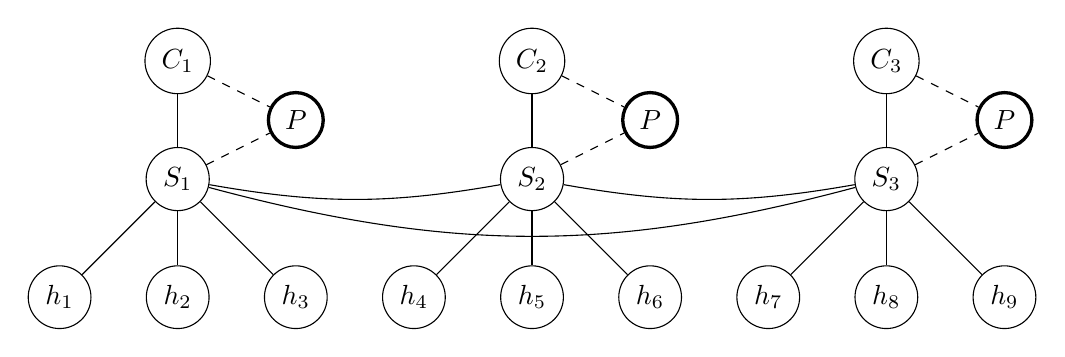
\begin{tikzpicture}[every node/.style={draw, circle},x=0.75cm,y=0.75cm]

    % For each switch ...
    \foreach \n in {1,2,3} {
      \pgfmathsetmacro\x{(\n-2)*6}
      \node (ctrl\n) at (\x ,  2) {$C_\n$};
      \node (S\n)    at (\x ,  0) {$S_\n$};

      \draw (S\n) -- (ctrl\n);

      % Paxos node
      \node [very thick] (P\n) at (\x + 2, 1) {$P$};
      \draw [dashed] (S\n) -- (P\n);
      \draw [dashed] (ctrl\n) -- (P\n);

      % For each host ...
      \foreach \h in {1,2,3} {
        \pgfmathsetmacro\pos{(\h - 2)*2}
        \pgfmathtruncatemacro\num{((\n - 1)*3) + int(\h)}

        % Host node
        \node (h\num) at (\x + \pos, -2) {$h_{\num}$};
        \draw (S\n) -- (h\num);
      }
    }

    % Links between switches
    \draw (S1) to[out=-10,in=190] (S2);
    \draw (S2) to[out=-10,in=190] (S3);
    \draw (S1) to[out=-15,in=195] (S3);

  \end{tikzpicture}
  \caption{Paxos ($P$) on the switches $S_1, S_2, S_3$ mitigates the need for special code on the servers.}
  \label{figure:paxos.on.switches}
\end{figure}

In figure \ref{figure:paxos.on.switches}, the switches themselves (and their
controllers) enable
support for Paxos.\footnote{We have moved the servers to several switches
to indicate a distributed nature between the switches.
Paxos on a single switch would not be very useful, as that would be a single
point of failure and---after all---be the sole decision point for message
ordering.}
This should let the servers be oblivious of the fact that Paxos is used to
enable ordering of packet arrival to them.

Besides, Paxos is now run at a much lower networking level and at the point
where switching is done---there will be less hops for each packet.

Of course, there are pros and cons for each scenario.
When implementing Paxos, one can often take advantage of
the particular way each server operates. Sometimes one actually
\textit{needs} to know this to implement Paxos.  Therefore, an
implementation of Paxos in each server's code base would be beneficial.

On the other hand, in our scenario, we can potentially add support for
message ordering through Paxos on servers that does not already support it.
The kinds of services that this would work on is for systems that are
deterministic in nature: The same input (or client packet) on any server
would produce the same internal state and output.
%
But there is a big class of software that has this behaviour:  Key-value
stores, logging servers, relational databases and so on.\footnote{But not
lock servers, because a lock can only be held by one server at a time.}

The only thing our model does not cover is the situation where a switch goes
completely down.  In that case, each connected server should start
synchronizing their internal state with any of the others that have been up.

All in all, we believe this is a viable experiment with practical benefits.
Indeed, using a software-based approach for switches lets us test our model
on \textit{any} existing piece of server software.

Moreover, we also intend to show how one can optimize the performance of
this model further, by moving parts of the Paxos implementation down into
the switches' flow tables.  This should have a big impact, because Paxos
handling is done at a lower level and closer to the central network
components than what would be the case with Paxos in the server code base.

\todo{Føler vi trenger flere, sterkere argumenter.}

  \chapter{Theory}

\section{Software--defined networking}

\section{OpenFlow}

\section{Paxos}

  \chapter{The non--Byzantine Paxos consensus algorithm}
\section{Paxos pseudo--code}

Algorithm \ref{algorithm:paxos.full.proposer} is for the Paxos proposer
role.  \texttt{TRUST}--messages are received during phase 1a, and
\texttt{PROMISE}s are received during phase 2a \cite{Lam01}.
The algorithms are a slight variation of the ones given in
\cite{Insane.Paxos}.

\begin{algorithm}
  \caption{Classic crash Paxos --- Proposer $c$ (leader)}
  \label{algorithm:paxos.full.proposer}
  \begin{algorithmic}

    \State $A$ \Comment{Set of acceptors}
    \State $crnd \gets 0$ \Comment{Current round (unique)}
    \State

    \On{$\langle \texttt{TRUST}, c \rangle$}{$\Omega_c$}
      \State $crnd \gets \textbf{pickNext}(crnd)$ \Comment{Phase 1a}
      \State $MV \gets \emptyset$ \Comment{Set of $\langle round, vote\ value \rangle$ tuples}
      \State \SendTo{$\langle \texttt{PREPARE}, crnd \rangle$}{$A$}
    \EndOn
    \State

    \On{$\langle \texttt{PROMISE}, rnd, vrnd, vval \rangle$}
       {$\text{acceptor}\ a$} \Comment{Phase 2a}
      \If{$rnd = crnd$}
        \State $MV \gets MV \cup \langle vrnd, vval \rangle$
        \If{$|MV| \geq n_a - t_a$}
          \If{$(vrnd = \bot)\ \forall\ \langle vrnd, vval \rangle \in MV$}
            \State $cval \gets \textbf{pickAny}()$
          \Else
            \State $cval \gets \textbf{pickLargest}(MV)$
          \EndIf
         \State \SendTo{$\langle \texttt{ACCEPT}, crnd, cval \rangle$}
                       {$A$}
        \EndIf
      \EndIf
    \EndOn

  \end{algorithmic}
\end{algorithm}

First is the initialization for the proposer. It has access to the set of
all acceptors $A$.  It also sets the current round number $crnd$ to
zero, but it must be a unique value per Paxos node.
Equations \ref{equation:crnd_i} and \ref{equation:crnd_mod_N} show how we
obtain a sequence of unique numbers.

Upon receiving a \texttt{TRUST} message from $\Omega_c$, it will pick the
proposal number larger than $crnd$, reset the set of
$\langle round, vote~value\rangle$ tuples and then send a
\texttt{PREPARE} message to all acceptors $A$.  Finally, it will
send a \texttt{PREPARE} message to all acceptors.

\begin{algorithm}
  \caption{Classic crash Paxos --- Acceptor $a$}
  \label{algorithm:paxos.full.acceptor}
  \begin{algorithmic}
    \State $P$ \Comment{Set of proposers}
    \State $L$ \Comment{Set of learners}
    \State $rnd \gets 0$ \Comment{Highest round seen}
    \State $vrnd \gets \bot$ \Comment{Round in which value was last accepted}
    \State $vval \gets \bot$ \Comment{Value last accepted}
    \State

    \On{$\langle \texttt{PREPARE}, n \rangle$}
       {$\text{proposer}\ c$} \Comment{Phase 1b}
      \If{$n > rnd$}
         \State $rnd \gets n$
         \State \SendTo{$\langle \texttt{PROMISE}, rnd, vrnd, vval\rangle$}
                       {$c$}
      \EndIf
    \EndOn
    \State

    \On{$\langle \texttt{ACCEPT}, n, v \rangle$}
       {$\text{proposer}\ c$} \Comment{Phase 2b}
      \If{$n \geq rnd \wedge n \neq vrnd$}
        \State $rnd \gets n$
        \State $vrnd \gets n$
        \State $vval \gets v$
        \State \SendTo{$\langle \texttt{LEARN}, n, v \rangle$}
                      {$L$}
      \EndIf
    \EndOn
  \end{algorithmic}
\end{algorithm}


\section{Simplifying the Paxos implementation}

In this chapter we will look at a simplified implementation of Paxos as
given in algorithms \ref{algorithm:paxos.full.proposer} and
\ref{algorithm:paxos.full.acceptor}.

It has been simplified to serve our needs, i.e.~to be able to handle
\texttt{ACCEPT} and \texttt{LEARN}--messages.  We can therefore remove the
$vrnd$ altogether.  Also, each Paxos node in our system will take on all
three roles, so we don't need separate sets for the acceptors, learners and
proposers. We will instead use simply $N$ for the set of Paxos nodes.

We need $crnd$ to be a sequence of unique values per Paxos node.
Instead of initializing it to zero, we will set it to the node's
unique ID.  Then, in $\textbf{pickNext}$, we will simply increment $crnd$
with the total number of Paxos nodes in the system.  This is a common trick
to ensure that each and every $crnd$ will be unique in the system and has
the added benefit that we can deduce the node ID by taking
$crnd\ (\bmod\ |N|)$, or taking the $crnd$ modulus the number of Paxos nodes
$|N|$ in the system:

Given
\begin{gather}
  crnd_i = \left\{
             \begin{array}{ll}
               n_{id} & \mbox{for } i = 0 \\
               crnd_{i-1} + |N| & \mbox{for } i \geq 1
             \end{array}
           \right. , n \in N
  \label{equation:crnd_i}
\end{gather}
then
\begin{gather}
  n_{id} \equiv crnd\ (\bmod\ |N|)\ \text{for}\ n \in N
  \label{equation:crnd_mod_N}
\end{gather}

where $n$ is the node and $N$ is the set of all nodes.  This leads to our
definition of $\textbf{pickNext}$ in algorithm
\ref{algorithm:paxos.simplified.pickNext}.

\begin{algorithm}
  \caption{Definition of \textbf{pickNext} based on equation \ref{equation:crnd_mod_N}}
  \label{algorithm:paxos.simplified.pickNext}
  \begin{algorithmic}
    \State $N$ \Comment{The set of all Paxos nodes}
    \State $n_{id} \gets \text{Unique Paxos node id}$
    \State $crnd \gets n_{id}$ \Comment{Replaces initialization of $crnd$ in algorithm \ref{algorithm:paxos.full.proposer}}
    \State
    \Function{$\textbf{pickNext}$}{}
      \State $\textbf{return}\ crnd + |N|$ \Comment{Unique per equation \ref{equation:crnd_mod_N}}
    \EndFunction
  \end{algorithmic}
\end{algorithm}

As we only intend to show that we can implement \texttt{ACCEPT} and
\texttt{LEARN}, we can ignore \texttt{TRUST}, \texttt{PROMISE} and
\texttt{PREPARE}--messages.  This leaves us with a very simple algorithm.

\begin{algorithm}
  \caption{Simplified algorithm for processing \texttt{ACCEPT}--messages}
  \label{algorithm:paxos.simple.acceptor}
  \begin{algorithmic}
    \State $N$\Comment{The set of Paxos nodes}
    \State $rnd \gets 0$ \Comment{Current round number}
    \State $vval \gets \bot$ \Comment{Packet ID of last round}
    \State

    \On{$\langle \texttt{ACCEPT}, n, v \rangle$}{$leader$}
      \If{$n \geq rnd$} % \wedge n \neq vrnd$}
        \State $rnd\gets n$
        \State $vval\gets v$ \Comment{The client packet ID}
        \ForIn{$node$}{$N$}
           \State \SendTo{$\langle \texttt{LEARN}, n, v \rangle$}
                         {$node$}
        \EndForIn
      \EndIf
    \EndOn
  \end{algorithmic}
\end{algorithm}

As for handling \texttt{LEARN}--messages, we can proceed to send the last
fragment of the client packet to the end--hosts when we have received a
learn from a majority.

\begin{algorithm}
  \caption{Simplified algorithm for processing \texttt{LEARN}--messages}
  \label{algorithm:paxos.simple.learner}
  \begin{algorithmic}
    \State $H$ \Comment{The set of end--hosts connected to this switch}
    \State

    \On{$\langle \texttt{LEARN}, n, v \rangle$}{$acceptor$}
      \If{$got\_{}majority(n)$}
        \ForIn{$host$}{$H$}
          \State \SendTo{$ last\_{}fragment(v) $}{$host$}
        \EndForIn
      \EndIf
    \EndOn
  \end{algorithmic}
\end{algorithm}

\section{Implementing simplified Paxos in Forth}

We will implement algorithms \ref{algorithm:paxos.simple.acceptor} 
and \ref{algorithm:paxos.simple.learner} in a combination of OpenFlow
matches and Forth.

\subsection{Paxos message packets}

For transmitting Paxos messages between the switches, we don't need to use
the IP--protocol.  A nice trick in OpenFlow is just to use Ethernet packets
and identify them by marking the Ethernet type field with a special value.
The packet payload will then consist of consecutive 32--bit values: The type of
Paxos message (\texttt{ACCEPT} or \texttt{LEARN} and their parameters.
This will make it easy for the switches to extract the contents.
Of course, since we don't use IP, we can only exchange these packets on a
local network.  If we wanted to distribute the switches across the network,
we would have to use IP.

\begin{table}[H]
  \begin{tabular}{|l|l|l|l|l|}
    \hline Ethernet header & Ethernet type & \ldots & Paxos message type & Payload \\
    \hline \ldots & \texttt{PAXOS} & \ldots & \texttt{HELLO} & $ \langle node_{id} \rangle $ \\
    \hline \ldots & \texttt{PAXOS} & \ldots & \texttt{ACCEPT} & $ \langle n, v \rangle $ \\
    \hline \ldots & \texttt{PAXOS} & \ldots & \texttt{LEARN} & $ \langle n, v \rangle $ \\
    \hline
  \end{tabular}

  \caption{The structure of Paxos message in Ethernet packets}
  \label{table:paxos.ethernet.packet}
\end{table}
\todo{We need to add more Ethernet frame/packet headers here}

If we intended to implement full Paxos, we could simply add more message
types to the above structure.

\subsection{OpenFlow matching rules}

We need several OpenFlow matching rules for this to work.

First, when a switch gets a client request (a packet from the WAN) it needs
to add flow table entries that forwards the packet to the leader.

When the system starts up, the switches need to announce themselves to each
other and learn which ports they are on.  For this we use the
\texttt{HELLO}--message given in table \ref{table:paxos.ethernet.packet}.
In a full Paxos implementation, the system would then perform leader
election.  That is out of scope for this thesis, so we will just designate
the first switch as the leader.  We also simplify the system further by
letting each switch know ahead how many other Paxos nodes there are---and
this will be static throughout the lifetime of the system\footnote{A full
Paxos implementation would also implement functionality for keeping tabs
on the liveness of each node.  OpenFlow has some limited support of
notifying the controllers when link status changes.  Also, a
production--quality system would allow for nodes to join and leave the
system.}.

\begin{table}[H]
  \begin{tabular}{|l|}
    \hline \textbf{Flow table entry} \\
    \hline Forward client requests to leader \\
    \hline
  \end{tabular}

  \caption{OpenFlow flow table entries}
  \label{table:paxos.flowtable.entries}
\end{table}

We also need entries for matching Paxos messages and react on these.
This is done by inserting entries that match on Ethernet type
\texttt{PAXOS} and ingress port from the leader.
The action will be to go to a new entry that looks at what kind of Paxos
message we have received\footnote{An optimization trick would be to
combine the Paxos packet type identifier with the Paxos message type and put
them both in the Ethernet type field.  Then we could use existing OpenFlow
matching instead of having to extract the Paxos message type.}.

Finally, when matching on Paxos message types, we would execute the Forth
bytecode and forward packets based on the return value from the code.

\subsection{New OpenFlow actions}

\todo{List opp nye actions her}
For the system to perform well, we don't want to store client packets in the
switch or the controller.  Instead, it would be nice if we could just pass
along client packets directly down to the end--hosts.

However, this means that the hosts will process the packets before we have a
chance to perform Paxos ordering.

We propose a neat solution to this problem.  When a switch receives a client
message, it will immediately perform IP--fragmentation of the message and
send the first fragment to the hosts.  The hosts networking stack will then
buffer the packet and wait for the last fragment.

When the Paxos consensus algorithm terminates, we will send the last
fragment down to the host, which will then pass the packet up the stack to
the server program.

We still need to store fragments, but if we choose the fragmentation offset
wisely, we need only store very small fragments.

The downside to this is that we break MTU rules, and some systems may behave
strange---or not at all.  But for our purposes we think this is a good
solution.

For this we need some new OpenFlow actions for fragmenting packets, storing
them and then forwarding the stored remaining fragment.

\begin{table}[H]
  \begin{tabular}{|l|l|l|}
    \hline \textbf{Action} & \textbf{Parameters} & \textbf{Description} \\
    \hline Fragment packet & buffer id, fragment offset & ... \\
    \hline Defragment packet & buffer id, buffer id & ... \\
    \hline Store fragment in table & buffer id & ... \\
    \hline Retrieve fragment from table & buffer id & ... \\
    \hline
  \end{tabular}

  \caption{New OpenFlow actions}
  \label{table:openflow.new.actions}
\end{table}

We also need new OpenFlow protocol messages so that the controller is able
to install flows with these new actions.  However, because of the scope of
this thesis, we will simply store these actions directly in OpenVSwitch and
pretend that these actions and flow entries came from the
controller\footnote{While trivial, this takes a little work to do fully.
One would first have to modify the OpenFlow protocol with new actions,
implement them and then do the same modifications on the controller.}.

\subsection{The switch data table}

Since each Paxos node needs to remember values for the round number, number
of nodes and so on, we propose that we add a simple table to each switch.

This is done by modifying the OpenVSwitch source code.

To conserve memory, we propose that each switch gets a table with 256
entries containing 32--bit values, for a total of 1024 bytes of memory.

OpenVSwitch needs to expose internally functions for manipulating this table
to Forth.  Our Forth code can then store the node id at location 0, round
numbers at location 1 and so on.

\subsection{Paxos message handlers in Forth}

Here we will define the Forth code for the Paxos message handlers.

\begin{verbatim}
variable crnd
variable node_id
variable vval
variable |N|

: pickNext ( -- crnd + |N| )
    \ Calculate the next value of crnd
    crnd @ |N| @ + ;

: on_accept ( n v -- 0 or -1 )
    over dup      ( n v -- v n n )
    rnd @ >= if   ( v n n -- v n )
        rnd !     ( v n -- v )
        vval !    ( v -- )
        -1        \ Return value TRUE
    else
        drop drop ( v n -- )
        0         \ Return value FALSE
    then ;
\end{verbatim}

\subsection{Why Forth?}

\todo{Insert a "defense" of why we chose Forth, and why we didn't implement
everything in OpenFlow}

What we want to avoid is to implement a complete, Turing--complete
programming language on the switch.  If that was our intention, we should
simply have used a platform that already had that, like Intel's NetVM
platform or NetFPGA\todo{Finn ut om flere alternative, og sjekk opp at disse
  nevnte er aktuelle}.

Instead, what we want is to provide \textit{simple} primitives that can be
implemented to run \textit{efficiently} on the hardware---requiring little
memory and few cycles per operation---while still being useful for other
networking protocols. (back up this statement on the last part)

In fact, our solution can, in fact, be implemented in a branchless manner on the
switch CPU, meaning that one can fill up the instruction pipeline for
maxiumem performance.  Our tables are simple vectors, meaning they
have constant time read and write operations and use little memory
(giving the benefit of improved memory locality).  In addition, the
low--level read and write instructions require extremely few cycles to run.

We think this is a good implementation for fastidious hardware implementors.

\subsection{Example of a full networking flow}

Now we will look at how an example client request will flow through the
system.

First the client sends an IP--packet to a switch.
The switch will then fragment the packet, send the first and largest
fragment to its hosts and forward it to all the other switches\todo{Dette er
litt annerledes. Og vi må sørge for at når de to andre switchene får
pakken så sender de den ikke videre}.

The end--hosts will receive an IP--fragment, store it and wait for the
remaining fragment.

When the leader receives a client packet, it will initiate the Paxos
algorithm.  In our simplified version of Paxos, it will then send
\texttt{ACCEPT} messages to the other two switches.

These switches will then send out \texttt{LEARN}--messages.
When a switch has received a majority of \texttt{LEARN}s, it will proceed to
send the last fragment down to its hosts.  The hosts will then combine the
fragments and pass the packet to the application.

The applications will then process the packet and, optionally, send back a
reply.\todo{Skal vi se bort fra hvordan vi velger ut svar fra endesystemene
og sender svar til klienten? Eller skal vi bare legge inn flows sånn at
kun den som mottok opprinnelig pakke kan svare klienten?}

\todo{Legg inn illustrasjoner her}

What we have accomplished here is using Paxos for ordering the client
requests down to the hosts, so that each host will receive packets in the
same order.  To test this, we will run simulations where several clients
send requests to the hosts. After some time, the state of each host should
be equal to each other.


\section{Paxos on the controller}

Our first step will be to implement simple Paxos \cite{Lam01} entirely in a
controller\index{controller}.

The aim is to show that a topology with a Paxos--enabled controller will
satisfy the requirements of Paxos --- i.e.,~that nodes in the network reach
consensus with progress\todo{Skriv om, og sjekk at forklaring på reqs er
riktig}.

We will use Mininet\index{Mininet} \cite{Lantz:2010:NLR:1868447.1868466} to
run and simulate the \ac{SDN} and POX\index{POX} \cite{POX.1} for
implementing a Paxos in an OpenFlow controller.  POX is part of the
NOX\index{NOX}--project \cite{Gude:2008:NTO:1384609.1384625}.  They both use
Python\index{Python}\footnote{Mininet uses Python version 2.7.}
\cite{vanRossum:2009:PRM:1610526} as the implementation language, which
means we can share some code between them.  Both projects are mature and
easy to use.  The Mininet simulation itself will run on a virtual machine
using VirtualBox\index{VirtualBox} \cite{Watson:2008:VBB:1344209.1344210}.


  \chapter{Design}
\label{chapter:design}

In this chapter, we will establish a solid design for our solution.

We will start by presenting a network topology for a replicated system using
Paxos on the switch.  After that, we will look at what OpenFlow can offer us
to implement our system, then design a system of flows that will provide a
replication system using Paxos.

\section{Topology}

A premise for for implementing Paxos in the switch is that we also deploy
multiple switches to provide the necessary resilience to failures.
%
Thus we need to provision a switch topology.

In this section, we will present how we plan to achieve this.
%
Starting with a single switch, we show how it can use a controller to
shuttle packets between clients and services running on end-hosts (figure
\ref{figure:graph.single.switch}).
%
By linking three such switches together, one will typically want to install
Paxos middleware on each host to provide service replication and
fault-tolerance (figure \ref{figure:paxos.on.servers}).
%
We then propose that by moving Paxos from the hosts to the switches, one can
offer the guarantees of Paxos, \textit{transparently}, for a wide class of
services (figure \ref{figure:paxos.on.switches}).

Let us start with the simplest case: One switch.\index{Paxos!topology}

In figure \vref{figure:graph.single.switch}, a switch $S_1$ is connected to
several nodes through ports.  On one of these, the switch will receive
packets from a set of clients $c_1$, $c_2$, $\dots$, $c_n$.
%
It has an OpenFlow controller $C_1$ and three end-hosts $h_1$, $h_2$ and
$h_3$ running software services.

\begin{figure}[H]
  \centering
  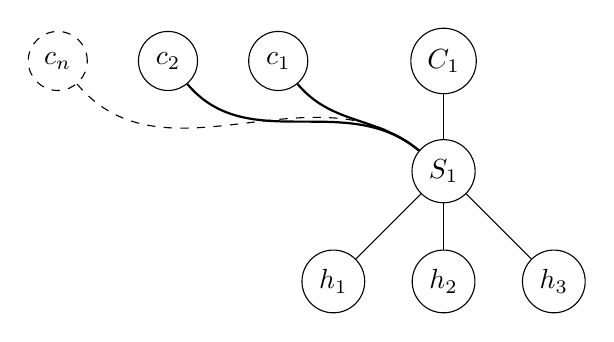
\begin{tikzpicture}[
      every node/.style={draw, circle, minimum width=0.75cm},
      x=0.7cm,
      y=0.7cm]
    \node (c1)    at (-3,  2) {$c_1$};
    \node (c2)    at (-5,  2) {$c_2$};
    \node [dashed] (cn) at (-7, 2) {$c_n$};

    \node (ctrl1) at ( 0,  2) {$C_1$};
    \node (S1)    at ( 0,  0) {$S_1$};
    \node (h1)    at (-2, -2) {$h_1$};
    \node (h2)    at ( 0, -2) {$h_2$};
    \node (h3)    at ( 2, -2) {$h_3$};

    \draw [thick] (c1) to[out=310,in=140] (S1);
    \draw [thick] (c2) to[out=310,in=140] (S1);
    \draw [dashed] (cn) to[out=310,in=140] (S1);

    \draw (S1) -- (ctrl1);
    \draw (S1) -- (h1);
    \draw (S1) -- (h2);
    \draw (S1) -- (h3);

  \end{tikzpicture}
  \caption{A single switch $S_1$ with its controller $C_1$, connected
    to end-hosts $h_1$, $h_2$, $h_3$ and clients $c_1$, $c_2$, $\dots$, $c_n$
    through ports.}
  \label{figure:graph.single.switch}
\end{figure}

Note that the actual location of the clients is irrelevant to our current
discussion.  Our focus is on the possible merits of placing Paxos on the
switch, not on how clients are able to reach the services. We will therefore
\textit{assume} that we are able to communicate with a set set of clients on
a designated port.

The topology in figure \vref{figure:graph.single.switch} allows us to
program the controller to replicate client messages to all its hosts.
%
It can do this by rewriting packets to match each host's address and
consolidate their replies.
%
While this should work well for \acs{UDP}\index{UDP!replication}, which is
stateless\index{stateless}, it would be markedly more involved with
\acs{TCP}\index{TCP!replication}.  We discuss this in chapter
\vref{chapter:tcp.replication}.

However, a single switch is inherently prone to failure.  Should it fail, it
would take down all the services along with it.
%
The obvious step is to add more switches.
%
Adding a second switch will not be sufficient, however, because if one of
them fails, we are left with a single point of failure.  It will also not be
enough to form a \textit{quorum}, which is required by Paxos.  Therefore, we
must add two additional switches.

\begin{figure}[H]
  \centering
  \begin{tikzpicture}[every node/.style={draw, circle},x=0.7cm,y=0.7cm]
    \foreach \n in {1,2,3} {
      \pgfmathsetmacro\x{(\n-2)*6}
      \node (c\n)    at (\x - 2,  2) {$c_\n$};
      \node (ctrl\n) at (\x ,  2) {$C_\n$};
      \node (S\n)    at (\x ,  0) {$S_\n$};

      \draw (c\n) to[out=305,in=125] (S\n);
      \draw (S\n) -- (ctrl\n);

      \foreach \h in {1,2,3} {
        \pgfmathsetmacro\pos{(\h - 2)*2}
        \pgfmathtruncatemacro\num{((\n - 1)*3) + int(\h)}
        \node (h\num) at (\x + \pos, -2) {$h_{\num}$};
        \draw (S\n) -- (h\num);
      }

    }

    % Links between switches
    \draw (S1) to[out=-10,in=190] (S2);
    \draw (S2) to[out=-10,in=190] (S3);

    % Fail-over links
    % c1
    \node [draw=none] (c1up) [above of=c1] {};
    \draw [dashed] (c1) to[out=90,in=270] (c1up);

    % c2
    \node [draw=none] (c2up) [above of=c2] {};
    \draw [dashed] (c2) to[out=90,in=270] (c2up);

    % c3
    \node [draw=none] (c3up) [above of=c3] {};
    \draw [dashed] (c3) to[out=90,in=270] (c3up);

    % S1 -- S3
    \draw [dashed] (S1) to[out=-15,in=195] (S3);

  \end{tikzpicture}
  \caption{Three switches $S_1, S_2, S_3$ with controllers $C_1, C_2, C_3$ acting as Paxos nodes.
           The dashed line between $S_1$ and $S_3$ is a potential fail-over
             link.  Each client is assumed to be able to connect to any
             switch.}
  \label{figure:graph.three.switches}
\end{figure}

In figure \vref{figure:graph.three.switches} we have three switches.
We have also indicated a possible fail-over link with a dashed line, in case
one switch fails.  Again, we disregard possible failures on the client-side.

We still want to perform replication of the services.  But now our latencies
are asymmetrical; a packet from $c_1$ will most likely take more time to
reach $h_9$ compared to $h_1$.
%
To mitigate this problem, we need to make sure that packets are delivered in
the same order to all hosts.  For this, we have chosen to look at Paxos.

\begin{figure}[H]
  \centering
  \begin{tikzpicture}[every node/.style={draw, circle},x=0.7cm,y=0.7cm]

    % For each switch ...
    \foreach \n in {1,2,3} {
      \pgfmathsetmacro\x{(\n-2)*6}
      \node (ctrl\n) at (\x ,  2) {$C_\n$};
      \node (S\n)    at (\x ,  0) {$S_\n$};

      \draw (S\n) -- (ctrl\n);

      % For each host ...
      \foreach \h in {1,2,3} {
        \pgfmathsetmacro\pos{(\h - 2)*2}
        \pgfmathtruncatemacro\num{((\n - 1)*3) + int(\h)}

        % Host node
        \node (h\num) at (\x + \pos, -2) {$h_{\num}$};
        \draw (S\n) -- (h\num);

        % Paxos node
        \node [very thick] (P\num) at (\x + \pos, -3.75) {$P$};
        \draw [dashed] (h\num) -- (P\num);
      }
    }

    % Links between switches
    \draw (S1) to[out=-10,in=190] (S2);
    \draw (S2) to[out=-10,in=190] (S3);
    \draw [dashed] (S1) to[out=-15,in=195] (S3);

  \end{tikzpicture}
  \caption{Support for Paxos on the servers $h_1, \dots, h_3$ requires a
    copy of the Paxos code $P$ on each server.}
  \label{figure:paxos.on.servers}
\end{figure}

Figure \vref{figure:paxos.on.servers} shows how most systems deploy Paxos
today.  

Each host acts as a Paxos node, having implemented it in their service
code-base.  This has several implications.

\todo{Se her}
List opp: Antall noder (ikke så viktig), at det skjer på høyt nivå i network
stakken, at de må spesialkode inn paxos, designe systemet med tanke på det,
osv.

Each service needs to have an implementation of Paxos in code (shown as
$P$ in figure \ref{figure:paxos.on.servers}).  It means the software
developer has to specifically add support for Paxos when designing the
server code, tailoring it for the particular service.  All Paxos handling
must be done at a high networking layer\index{networking layers}---most
likely in the application layer\index{application layer} at the very top.

Now consider the situation where the switch provides Paxos
capabilities\index{Paxos!on switch} (figure \ref{figure:paxos.on.switches}).

\begin{figure}[H]
  \centering
  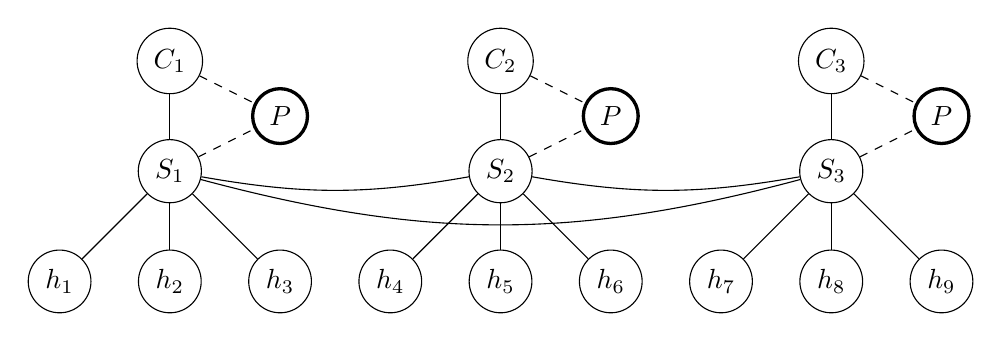
\begin{tikzpicture}[every node/.style={draw, circle},x=0.7cm,y=0.7cm]

    % For each switch ...
    \foreach \n in {1,2,3} {
      \pgfmathsetmacro\x{(\n-2)*6}
      \node (ctrl\n) at (\x ,  2) {$C_\n$};
      \node (S\n)    at (\x ,  0) {$S_\n$};

      \draw (S\n) -- (ctrl\n);

      % Paxos node
      \node [very thick] (P\n) at (\x + 2, 1) {$P$};
      \draw [dashed] (S\n) -- (P\n);
      \draw [dashed] (ctrl\n) -- (P\n);

      % For each host ...
      \foreach \h in {1,2,3} {
        \pgfmathsetmacro\pos{(\h - 2)*2}
        \pgfmathtruncatemacro\num{((\n - 1)*3) + int(\h)}

        % Host node
        \node (h\num) at (\x + \pos, -2) {$h_{\num}$};
        \draw (S\n) -- (h\num);
      }
    }

    % Links between switches
    \draw (S1) to[out=-10,in=190] (S2);
    \draw (S2) to[out=-10,in=190] (S3);
    \draw (S1) to[out=-15,in=195] (S3);

  \end{tikzpicture}
  \caption{Paxos ($P$) on the switches $S_1, S_2, S_3$ mitigates the need for special code on the servers.}
  \label{figure:paxos.on.switches}
\end{figure}

In figure \ref{figure:paxos.on.switches}, the switches themselves (and their
controllers\index{Paxos!controller}) enable
support for Paxos.\footnote{We have moved the servers to several switches
to indicate a distributed nature between the switches.
Paxos on a single switch would not be very useful, as that would be a single
point of failure and---after all---be the sole decision point for message
ordering.}
This should let the servers be oblivious of the fact that Paxos is used to
enable ordering of packet arrival to them.

Besides, Paxos is now run at a much lower networking level\index{networking
layers} and at the point where switching is done---there will be less hops
for each packet.

Of course, there are pros and cons for each scenario.
When implementing Paxos, one can often take advantage of
the particular way each server operates. Sometimes one actually
\textit{needs} to know this to implement Paxos.  Therefore, an
implementation of Paxos in each server's code base would be beneficial.

Also, it means that we need to run code on the switches themselves. This
gives rise to a wide range of non-functional requirements for the code.
For instance, code that runs for too long must be
preempted\index{preemption} to let the switch smoothly handle other
requests. Not doing so may result in packet loss, high latency or
worse---complete incapacity to serve data. Besides, switches do not normally
have hardware capable of running \textit{generic} software fast. They
usually have highly optimized hardware to do some of the heavy-lifting.

On the other hand, in our scenario, we can potentially add support for
message ordering through Paxos on servers that does not already support it.
The kinds of services that this would work on is for systems that are
deterministic in nature: The same input (or client packet) on any server
would produce the same internal state and output.
%
But there is a big class of software that has this behaviour:  Key-value
stores, logging servers, relational databases and so on.\footnote{But not
lock servers, because a lock can only be held by one server at a time.}

The only thing our model does not cover is the situation where a switch goes
completely down.
In that case, each connected server should start
synchronizing their internal state with any of the others that have been up.
\todo{Mangler jo også leader election og failures. Må få
  fram at jeg mener at KONSEPTET støtter mange ting, men ikke vår
    IMPLEMENTASJON.}

All in all, we believe this is a viable experiment with practical benefits.
Indeed, using a software-based approach for switches lets us test our model
on \textit{any} existing piece of server software.

Moreover, we also intend to show how one can optimize the performance of
this model further, by moving parts of the Paxos implementation down into
the switches' flow tables.  This should have a big impact, because Paxos
handling is done at a lower networking layer and closer to the central network
components than what would be the case with Paxos in the server's code.


\section{Capabilities in OpenFlow}
\label{chapter:details.openflow}

Now that we have discussed the main algorithms and our simplification of
them, we must take a look at what OpenFlow can offer us to reach our goals.

\todo{Show ONLY openflow 1.3, possibly 1.4}

To see how we can enable Paxos functionality in OpenFlow, we need to take a
look at what features it can provide us.  There are several versions of the
OpenFlow specification, so we'll review the differences in each
one.\footnote{Unfortunately, the most widely supported version of OpenFlow in
simulators and controllers seem to be OpenFlow version 1.0.}

Naturally, we could implement the whole Paxos algorithm in the controller
itself.  Doing so should be quite trivial: One could modify an existing
implementation and make it use OpenFlow to transmit packets between
switches.  However, that would be very inefficient compared to running the
entire algorithm, or parts of it, on the switch.

Prior to OpenFlow 1.0 \cite{openflow-1.0} there were several working
drafts not meant for implementation.  We will not look at these prior
versions.

In the tables below, you can see what version 1.0 offers in terms of core
functionality.  Some details have been omitted in favor of giving a clear
overview.  For details, see the full specification \cite{openflow-1.0}.

What's most important in 1.0, compared to later versions, is that it only
has \textit{one} flow table and only supports IPv4.  Other than that it has
counters per table, per flow, per port and per queue.  The headers that can
be used for matching packets are listed in table
\ref{table:openflow-1.0.headers} \vpageref{table:openflow-1.0.headers} and
the actions in table \ref{table:openflow-1.0.actions}
\vpageref{table:openflow-1.0.actions}.

By \textit{transport} address and port, we mean \ac{TCP} or \ac{UDP},
depending on what packet is currently matched\index{OpenFlow!transport}.

The specification requires compliant switches to update packet checksums
when modifying fields that require it.

\begin{table}
  \centering
  \begin{tabular}{l}
    \hline
     \textbf{Header-field} \\
    \hline
     Ingress port\index{OpenFlow!match on ingress port} \\

     Ethernet source address\index{OpenFlow!match on Ethernet} \\
     Ethernet destination address\index{OpenFlow!match on Ethernet} \\

     VLAN ID\index{OpenFlow!match on VLAN} \\
     VLAN priority\index{OpenFlow!match on VLAN} \\

     IP source address\index{OpenFlow!match on IP address} \\
     IP destination address\index{OpenFlow!match on IP address} \\
     IP protocol\index{OpenFlow!match on IP protocol} \\
     IP \ac{ToS} bits\index{OpenFlow!match on ToS} \\

     Transport source port\index{OpenFlow!UDP}\index{OpenFlow!TCP}\index{OpenFlow!transport} \\
     Transport destination port \\
    \hline
  \end{tabular}
  \caption{Header-fields that can be matched in OpenFlow 1.0.}
  \label{table:openflow-1.0.headers}
\end{table}
\index{OpenFlow!matching}
\index{OpenFlow!header-fields}
\index{OpenFlow!matching header-fields}

\begin{table}
  \centering
  \begin{tabular}{lll}
    \hline
      \textbf{Action} &
      \textbf{Required} &
      \textbf{Options} \\

    \hline
      Forward\index{OpenFlow!forwarding action} &
      Required &
               To all \\
     & & To controller \\
     & & To local switch \\
     & & To flow table \\
     & & To port \\
    \\
      Forward\index{OpenFlow!forwarding action} &
      Optional &
               Normal \\
     & & Flood\index{OpenFlow!flooding action} \\
    \\
      Enqueue\index{OpenFlow!enqueue action} &
      Optional &
      Can be used to implement, e.g., \acs{QoS}\index{OpenFlow!QoS} \\
    \\
      Drop\index{OpenFlow!drop action} &
      Required &
      Drop packet \\
    \\
      Modify-field\index{OpenFlow!modify-field action} &
      Optional &
               Set or replace VLAN ID\index{OpenFlow!modify VLAN} \\
     & & Set or replace VLAN priority\index{OpenFlow!modify VLAN} \\
     & & Strip any VLAN header\index{OpenFlow!modify VLAN} \\
     & & Replace Ethernet source address\index{OpenFlow!modify Ethernet addresses} \\
     & & Replace Ethernet destination address \\
     & & Replace IPv4 source address\index{OpenFlow!modify IPv4 addresses} \\
     & & Replace IPv4 destination address\index{OpenFlow!modify IPv4 addresses} \\
     & & Replace IPv4 \acs{ToS} bits\index{OpenFlow!modify ToS bits} \\
     & & Replace transport source port\index{OpenFlow!modify transport ports} \\
     & & Replace transport destination port\index{OpenFlow!modify transport ports} \\
    \hline
  \end{tabular}
  \caption{Actions in OpenFlow 1.0.}
  \label{table:openflow-1.0.actions}
\end{table}
\index{OpenFlow!actions}

\todo{Skriv litt mer om features i openflow-versjoner nyere enn 1.0, ikke
  lag tabeller, bare list opp store forskjeller. Bruk dette i
    argumentasjonen under.}

\section{Limitations in OpenFlow}

By looking at what OpenFlow versions 1.1--1.3\index{OpenFlow!versions} offer,
one can see that we can't really make use of any of the added functionality
for running Paxos.  What we need is the ability to run programs on the
switch, which is something OpenFlow does not support at all.  Neither do
their action primitives add up to anything that could be used for
remembering state (such as the current round number) or executing
if-then-else statements.

One possible solution would be to insert a lot of flow table entries that
each waited for a specific round number.  But that would not be an elegant
or practical solution.

They \textit{do}, however, offer us the ability to implement Paxos entirely
on the controller.  We have actually done this, but one of the stated goals
of this thesis was to move parts of the Paxos code down to the switch
itself.  For this we simply need to be able to run full Turing-equivalent
programming languages\index{programming language}.

For remembering state, we looked at the meta-data\index{OpenFlow!metadata}
that is available in later versions of OpenFlow.  However, metadata only
exists as the packet is processed in the pipeline of flow tables, and is
erased when the packet actions are applied at the end.  To remember state,
we will need to add a table to hold such data in the switch.

Finally, we have to look at which OpenFlow versions our software components
support.

Mininet seems to support whatever version of OpenFlow that Open vSwitch uses,
as this is what it uses as a switch.  Open vSwitch\index{Open vSwitch}
supports OpenFlow versions 1.0---1.3\index{Open vSwitch!OpenFlow support}
almost fully, but support for 1.4 is flaky, and may crash.  So 1.4 is out of the question.

The most obvious component to look at is POX\index{POX}, our controller framework in
Python, which only supports OpenFlow 1.0.\footnote{It does seem to support
some \textit{Nicira extensions}\index{Nicira}\index{OpenFlow!Nicira
extensions}, though.  These are extensions that were originally added to
early OpenFlow versions, but much of it has been implemented in later
versions.  There is also a fork of POX (and other software projects) written
by CPqD that adds support for newer OpenFlow versions, but we haven't looked
at it.}\todo{Vær sikker på at vi ikke kan gjøre dette i Nicira extensions.
Mener jeg har rett, men dobbelsjekk.}

But the major point for our decision is what OpenFlow can offer us.
There simply is no way of executing general code, and there is no way to
remember state.\footnote{We even investigated whether we could use the
counters to count round numbers or store them in IPv6 addresses, using VLAN
for storing data, etc.  All those ideas turned out to be very hairy to
implement, with a real possibility of not working correctly.}

All in all, we have decided to use OpenFlow 1.0 where applicable and extend
it where needed.  Using the flow table, controller and bytecode is a simple
but good, practical decision.

\todo{Ta vekk bytecode, forklar at det er irrelevant hva språk/type vi
  bruker}

\section{Decisions}

We have seen that OpenFlow does not offer the capabilities we need to
implement Paxos on the switch.  We could implement Paxos on the controller,
but that would be nearly equivalent to having adding Paxos to the software
running on the end-hosts.\todo{Dette argumentet må være mye sterkere.
  Vi må vise på en mer klar måte at vi ikke kommer utenom programmering.}

Thus, we have decided to use a combination of OpenFlow flow table rules and
programs running in Open vSwitch as bytecode\index{bytecode} compiled
fragments to handle the details of the Paxos
algorithms.\index{OpenFlow!bytecode}

\todo{Legg til selve designet her, siden tittelen sier det! Vis hvor vi
bruker flow tables (ikke vis detaljer, det kommer senere), vis
nettverksflyt, vis hvor bytecode blir eksekvert, og hva som kjører på
controller.}

\section{Choice of Switch Programming Language}

\todo{Ta vekk}

What we want is to provide \textit{simple} primitives that can be
implemented to run custom code \textit{efficiently} on the
hardware---requiring little memory and few cycles per operation---while
still being useful for other networking protocols.
\todo{back up this statement on the last part}

We think this is a good implementation for fastidious hardware implementers,
but \textit{any} programming language---preferably one that can produce
bytecode---would work just as fine.
\todo{Finn ut hvor jeg snakker om Ngaro og flytt tekst over her.}


\section{Paxos in OpenFlow}

To be able to run Paxos on the switch, we must first extend the OpenFlow
Switch Specification with a new \textit{Paxos action}.
\index{flows!Paxos action}\index{OpenFlow!Paxos action}%
\index{Paxos!OpenFlow action}%
%
This will allow us to freely \textit{compose} flows that run the
Paxos algorithm as one part of their actions.
%
Finally, we must modify Open vSwitch so that we can run the new action.

\subsection{Extending the OpenFlow Switch Specification}

As discussed earlier in chapter \ref{chapter:openflow.design}, it would be
impractical to attempt to use existing actions in the OpenFlow specification
to implement the Paxos algorithm.
%
The OpenFlow specifications, as of version 1.4 \cite{openflow-1.4}, are
backward-compatible, meaning that a newer OpenFlow version will support all
features in older ones.  We will therefore choose to extend version 1.0
\cite{openflow-1.0}, because it was the first public version and therefore
the most widely supported.

The idea is to add a new \textit{Paxos action} with a parameters 
specifying whether to run the \textit{On Client}, \textit{On Accept} or 
\textit{On Learn} parts of the Paxos algorithm given in chapter
\vref{ch:simplifying.paxos}.
%
As shown in \vref{chapter:openflow.background}, we can then specify
precisely what kind of events we want to trigger Paxos ordering for and
combine that with other actions, such as which port the output should go to.

The part of the specification we need to extend is the 
\textit{Flow Action Structures} \cite[pp.~21--22]{openflow-1.0},
which will be an \textit{optional} action \cite[pp.~3--6]{openflow-1.0}.
Listing \ref{listing:ofp10.action.type} shows the modification made to
the C\index{C} enumeration type \texttt{ofp10\_{}action\_{}type} from the Open
vSwitch source code,\footnote{The file
  \texttt{ovs/include/openflow/openflow-1.0.h}} which is nearly identical
to the official specification.

\begin{lstlisting}[
  caption={Adding the \texttt{OFPAT10\_{}PAXOS} action to the OpenFlow
           specification},
  label={listing:ofp10.action.type}]
enum ofp10_action_type {
    OFPAT10_OUTPUT,             /* Output to switch port. */
    OFPAT10_SET_VLAN_VID,       /* Set the 802.1q VLAN id. */
    OFPAT10_SET_VLAN_PCP,       /* Set the 802.1q priority. */
    OFPAT10_STRIP_VLAN,         /* Strip the 802.1q header. */
    OFPAT10_SET_DL_SRC,         /* Ethernet source address. */
    OFPAT10_SET_DL_DST,         /* Ethernet destination address. */
    OFPAT10_SET_NW_SRC,         /* IP source address. */
    OFPAT10_SET_NW_DST,         /* IP destination address. */
    OFPAT10_SET_NW_TOS,         /* IP ToS (DSCP field, 6 bits). */
    OFPAT10_SET_TP_SRC,         /* TCP/UDP source port. */
    OFPAT10_SET_TP_DST,         /* TCP/UDP destination port. */
    OFPAT10_ENQUEUE,            /* Output to queue. */
    OFPAT10_PAXOS,              /* Extension: Run Paxos algorithm. */
    OFPAT10_VENDOR = 0xffff
};
\end{lstlisting}

The Paxos action has only one parameter: Which part of algorithm
\ref{ch:simplifying.paxos} to run.  The structure of this parameter is given
in listing \ref{listing:ofp10.action.paxos} and its its possible values are
defined in table \ref{table:paxos.event.codes}.

\begin{lstlisting}[
  caption={The \texttt{OFPAT10\_{}PAXOS} parameters},
  label={listing:ofp10.action.paxos}]
struct ofp10_action_paxos {
    ovs_be16 type;            /* OFPAT10_PAXOS. */
    ovs_be16 len;             /* Length is 8. */
    ovs_be32 paxos_event;
};
OFP_ASSERT(sizeof(struct ofp10_action_paxos) == 8);
\end{lstlisting}

As we can see, \texttt{paxos\_{}event} is encoded using a big-endian, unsigned
32-bit integer.  Network protocols commonly use big-endian numbers.
%
Its possible values are given in table \ref{table:paxos.event.codes}.

\begin{table}[H]
  \centering
  \begin{tabular}{|l|l|}
    \hline
      \textbf{Value} &
      \textbf{Meaning}
      \\

    \hline
      \texttt{0x7A01} &
      Run ``On Accept'' (algorithm \ref{algorithm:paxos.simple.acceptor})
      \\

    \hline
      \texttt{0x7A02} &
      Run ``On Learn'' (algorithm \ref{algorithm:paxos.simple.learner})
      \\

    \hline
      \texttt{0x7A40} &
      Run ``On Client'' (see ch.~\ref{chapter:incoming.client})
      \\

    \hline
  \end{tabular}
  \caption{Possible values for \texttt{paxos\_{}event} in listing
           \ref{listing:ofp10.action.paxos}}
  \label{table:paxos.event.codes}
\end{table}

The values in table \ref{table:paxos.event.codes} have been chosen
somewhat arbitrarily to correspond to the Ethernet types given
in table \ref{table:paxos.ethernet.type.encoding}, chapter
\vref{chapter:paxos.message}.  They could have been simply zero, one
and two.  The point here is just to specify the \textit{encoding} 
used in the protocol.  We have chosen to use a width of 32-bits so
that the structure will be aligned on a word boundary, which is the
convention in the specification.

Because of the scope of this thesis, we have been practical in choosing only
\textit{one} parameter for the Paxos action.
%
In a production environment, one would likely need several more parameters.
%
For example, it could be useful to distinguish between different sets of
Paxos nodes so they could operate independently of each other, using
entirely different sets of round numbers and sequence numbers.
That would require another parameter and a corresponding change to
Open vSwitch.

Ta med:
  - the big picture, er det egentlig korrekt å gjøre en sånn endring
  i openflow? altså vi har ikke gjort dette for at vi foreslår at
  openflow faktisk --- for alle --- implementerer denne saken, men
  vi bruker det som piggy-backing for å teste ut dette på en
  komponerbar måte, så sånn sett så er det nydelig, og det kan
  lett testes med simulator, controllere osv for de støtter jo
  alleerede of
  - vedr ordering, vi har jo nå en kø som sender ut in order,
   dette er litt på kant med spekken (faktisk egentlig ikke,
       spekken sier ordering ikke er spesifisert, men vi har
       jo en side-effekt her som går kontra spekken, siden
       ting plutselig kan sendes ut senere).

\subsection{Modifying Open vSwitch}

Ta med:  hvorfor vi må endre ovs,
Features bit (kan annonsere features, de som ikke støtter paxos
bruker det ikke). TA med grovt hvor vi må endre (filer, kall),
litt om arkitekturen til ovs (datapath, odp, kernel modul osv), og ta med at vi bruker
ofctl til programmering istedenfor å bruke tid på POX.
Ta med at vi bruker odp for nå, men at vi har implementert (dvs dette kommer
i "implementation") i kernel også.

\subsection{Composing Flows to Implement Paxos Replication}

flow regler, flyt osv for å få paxos til å funke.


  \chapter{Implementation}
\label{chapter:implementation}

Based on the design in chapter \ref{chapter:design}, we will now look at
implementation details.

To be able to run Paxos in the switch, we must first extend the OpenFlow
Switch Specification with a new \textit{Paxos action}.
\index{flows!Paxos action}\index{OpenFlow!Paxos action}%
\index{Paxos!OpenFlow action}%
%
This will allow us to freely \textit{compose} flows that run the
Paxos algorithm as one part of their actions.
%
Finally, we must modify Open vSwitch so that we can run the new action.

\section{Extending the OpenFlow Specification}

As discussed earlier in chapter \ref{chapter:openflow.design}, it would be
impractical to attempt to use existing actions in the OpenFlow specification
to implement the Paxos algorithm.
%
The OpenFlow specifications, as of version 1.4 \cite{openflow-1.4}, are
backward-compatible, meaning that a newer OpenFlow version will support all
features in older ones.  We will therefore choose to extend version 1.0
\cite{openflow-1.0}, because it was the first public version and therefore
the most widely supported.

The idea is to add a new \textit{Paxos action} with a parameters 
specifying whether to run the \textit{On Client}, \textit{On Accept} or 
\textit{On Learn} parts of the Paxos algorithm given in chapter
\vref{ch:simplifying.paxos}.
%
As shown in \vref{chapter:openflow.background}, we can then specify
precisely what kind of events we want to trigger Paxos ordering for and
combine that with other actions, such as which port the output should go to.

The part of the specification we need to extend is the 
\textit{Flow Action Structures} \cite[pp.~21--22]{openflow-1.0},
and it will be an \textit{optional} action \cite[pp.~3--6]{openflow-1.0}.
%
Listing \ref{listing:ofp10.action.type} shows the modification made to
the C\index{C} enumeration type \texttt{ofp10\_{}action\_{}type} from the
Open vSwitch source
code.\footnote{\texttt{ovs/include/openflow/openflow-1.0.h}}
We have included listing listing:ofp10.action.type as-is because this is how
it is defined in the published OpenFlow specification \cite{openflow-1.0}.
%
The listing is identical to the official specification, except for the
number suffix in \texttt{OFPAT10}.

\begin{lstlisting}[
  caption={Adding the \texttt{OFPAT10\_{}PAXOS} action to the OpenFlow
           specification},
  label={listing:ofp10.action.type}]
enum ofp10_action_type {
    OFPAT10_OUTPUT,             /* Output to switch port. */
    OFPAT10_SET_VLAN_VID,       /* Set the 802.1q VLAN id. */
    OFPAT10_SET_VLAN_PCP,       /* Set the 802.1q priority. */
    OFPAT10_STRIP_VLAN,         /* Strip the 802.1q header. */
    OFPAT10_SET_DL_SRC,         /* Ethernet source address. */
    OFPAT10_SET_DL_DST,         /* Ethernet destination address. */
    OFPAT10_SET_NW_SRC,         /* IP source address. */
    OFPAT10_SET_NW_DST,         /* IP destination address. */
    OFPAT10_SET_NW_TOS,         /* IP ToS (DSCP field, 6 bits). */
    OFPAT10_SET_TP_SRC,         /* TCP/UDP source port. */
    OFPAT10_SET_TP_DST,         /* TCP/UDP destination port. */
    OFPAT10_ENQUEUE,            /* Output to queue. */
    OFPAT10_PAXOS,              /* Extension: Run Paxos algorithm. */
    OFPAT10_VENDOR = 0xffff
};
\end{lstlisting}

The Paxos action has only one parameter: Which part of algorithm
\ref{ch:simplifying.paxos} to run.  The structure of this parameter is given
in listing \ref{listing:ofp10.action.paxos} and its its possible values are
defined in table \ref{table:paxos.event.codes}.
%
All action structures are required to start with the \texttt{type} and
\texttt{len} fields.

\begin{lstlisting}[
  caption={The \texttt{OFPAT10\_{}PAXOS} parameters},
  label={listing:ofp10.action.paxos}]
struct ofp10_action_paxos {
    ovs_be16 type;            /* Required: OFPAT10_PAXOS. */
    ovs_be16 len;             /* Required: Length is 8. */
    ovs_be32 paxos_event;
};
OFP_ASSERT(sizeof(struct ofp10_action_paxos) == 8);
\end{lstlisting}

As we can see, \texttt{paxos\_{}event} is encoded as a big-endian, unsigned
32-bit integer.
%
Its possible values are given in table \ref{table:paxos.event.codes}.

\begin{table}[H]
  \centering
  \begin{tabular}{|c|l|c|l|}
    \hline
      \textbf{Value} &
      \textbf{Meaning} &
      \textbf{Algorithm} &
      \textbf{\texttt{ovs-ofctl} argument}
      \\

    \hline
      \texttt{0x7A01} &
      Run ``On Accept'' &
      \ref{algorithm:paxos.simple.acceptor} &
      \texttt{paxos:onaccept}
      \\

    \hline
      \texttt{0x7A02} &
      Run ``On Learn'' &
      \ref{algorithm:paxos.simple.learner} &
      \texttt{paxos:onlearn}
      \\

    \hline
      \texttt{0x7A40} &
      Run ``On Client'' &
      \ref{algorithm:paxos.simple.client} &
      \texttt{paxos:onclient}
      \\

    \hline
  \end{tabular}
  \caption{Possible values for \texttt{paxos\_{}event} in listing
           \ref{listing:ofp10.action.paxos}}
  \label{table:paxos.event.codes}
\end{table}

The values in table \ref{table:paxos.event.codes} have been chosen
to correspond to the Ethernet types given
in table \vref{table:paxos.ethernet.type.encoding}, although they
could have been simply zero, one and two.
%
The last column contains the command-line arguments that will be
accepted by \texttt{ovs-ofctl} when adding flows.

Because of the thesis scope, we have only added a single action parameter
\texttt{paxos\_type}.
%
In a production environment, however, one would likely need several more.
%
For example, it could be useful to distinguish between different
\textit{sets} of Paxos nodes so they could operate independently of each
other on the same network.
%
Here, we have only \textit{one} set of Paxos nodes who all have the same
leader.

\subsection{Modifications to Open vSwitch}

As mentioned in section \vref{chapter:mininet}, the component in our system
that actually executes OpenFlow actions is \textit{Open vSwitch}.
To fully implement the new Paxos OpenFlow action, we need to do this in Open
vSwitch.  Details can be found in section \vref{chapter:compiling.ovs}.

Looking at table table \vref{table:paxos.event.codes}, the rightmost column
(\textbf{\texttt{ovs-ofctl} argument}) contains arguments to the Open
vSwitch command-line tool \texttt{ovs-ofctl}, that can be used to program
Paxos actions as smaller parts of bigger flows.

To demonstrate how elegantly one can set up flows that use Paxos ordering,
consider the below example for installing a flow on the switch
\texttt{S1}.

\begin{Verbatim}
sudo ovs-ofctl add-flow S1 \
               in_port=3,dl_type=0x7a40,actions=paxos:onclient,output:5
\end{Verbatim}

The above command installs a new flow entry on \texttt{S1}, matching packets
coming in on port 3 with the Ethernet type \texttt{0x7a40}.  
Referring to table \vref{table:paxos.event.codes}, we see that this flow
will match on packets of type \texttt{CLIENT}.

Furthermore, under \texttt{actions=}, we instruct Open vSwitch to run the
Paxos action with the parameter \texttt{onclient}.  This means that for
matching packets, Open vSwitch will dispatch the packet to the \textit{on
client} function (the argument \texttt{paxos:onclient}), described in
chapter \vref{chapter:paxos.client.message} and algorithm
\vref{algorithm:paxos.simple.client}.
%
This algorithm will output an accept message to output port 5
(\texttt{output:5})
If we want to explicitly set the destination address of the packet, one can
just prepend the output with the modification action
\texttt{mod\_dl\_dst=a1:b2:c3:d4:e5:f6}.
To send out on several ports, one just needs to add more \texttt{output:<N>}
actions, or the packet can be flooded on all ports with
\texttt{output:flood}.

What we are doing here is programming the switch's flow table using Paxos
primitives as constituent elements.  For the actual implementation, we refer
to the appendix, section \vref{chapter:compiling.ovs}.

We have implemented all of the actions in table
\ref{table:paxos.event.codes}, including multi-Paxos storage of packets in
slots, but with the important exception of the queue processing (algorithm
\ref{algorithm:paxos.simple.learner}, section
\ref{ch:simplifying.paxos}).

The above command translates client packets to Paxos \texttt{ACCEPT}
packets.  For a Paxos node on another switch, we can simply use the
\texttt{paxos:onaccept} action.  Since switch $S_2$ of figure
\vref{figure:paxos.on.switches} may receive Paxos messages from both $S_1$
and $S_3$, we may want to only react on packets that are explicitly
addressed to $S_2$.
%
To do so, assuming the MAC-address is \texttt{22:22:22:22:22:22}, one may
simply add a matching pattern for it, along with the obligatory check for
the Ethernet type field corresponding to an accept message
(\texttt{0x7A01}):

\begin{Verbatim}
sudo ovs-ofctl add-flow S2 \
    dl_src=11:11:11:11:11:11,\         # match from leader S1
    dl_dst=22:22:22:22:22:22,\         # match S2 MAC-address
    dl_type=0x7a01,\                   # match ACCEPT message
    actions=paxos:onaccept,\           # run "On Accept"
    mod_dl_src=22:22:22:22:22:22,\     # set source MAC address
    mod_dl_dst=33:33:33:33:33:33,\     # set destination MAC to S3
    output:5,\                         # output to port 5
    mod_dl_dst=11:11:11:11:11:11,\     # set destination MAC to S1
    output:1                           # output to port 1
\end{Verbatim}

The flow above is an \textit{actual} flow that we used---and verified to
work---in our network simulator.  If all conditions of algorithm
\ref{algorithm:paxos.simple.acceptor} are met, this flow wil send out a
learn message to $S_1$ and $S_3$.

Comparing this with writing equivalent flows as procedures in Python, this
is \textit{vastly} easier to do.  An \textit{excerpt} from the code for
accept-hanling in the Python controller is given below.

\begin{lstlisting}[
  caption={Shortened excerpt of Python code for handling Paxos accept messages},
  label={listing:python.accept}]
def on_accept(self, event, message):
  n, seqno, v = PaxosMessage.unpack_accept(message)
  src, dst = self.get_ether_addrs(event)

  # From leader?
  if src != self.leader.mac:
    return EventHalt # drop message

  slot = self.state.slots.get_slot(seqno)

  if n >= self.state.crnd and n != slot.vrnd:
    slot.vrnd = n
    slot.vval = v

    # Send learns to all
    for mac in self.state.ordered_nodes(self.mac):
      self.send_learn(mac, n, seqno, self.lookup_port(mac))

  return EventHalt
\end{lstlisting}

The code in the listing above is a shortened version of the
actual implementation.
%
Of course, we have had to actually \textit{implement} the above code in
equivalent C code in Open vSwitch, but the big gain is that the flows are
happening on the switch, and requires no upcall to the controller.


\todo{Flytt resten av kapittelet}

As discussed in \vref{chapter:theory.flow.table}, well-designed controllers
should install flows incrementally as they learn the network topology.
%
We must therefore first implement a system that works entirely without flow
entries. (Dette er en del av design-diskusjon, vi skal bare implementere det
her).

Next, we will implement flows in the system. As discussed previously, this
requires an extension to the OpenFlow-protocol and the switch software we
use, Open vSwitch. \todo{Dette må ha vært diskutert før}

Mer tekst: At vi har, i designet, extenda OpenFlow + Open vSwitch slik at vi
kan kjøre kode. Vi viser implementasjonen her, husk å skille på design og
implementasjon klart og tydelig.

\label{implementation.simplified.paxos}

We will implement algorithms \ref{algorithm:paxos.simple.acceptor} 
and \ref{algorithm:paxos.simple.learner} in a combination of OpenFlow
matches\index{OpenFlow!matching} and its extensions that were introduced
in \vref{chapter:extending.openflow}.

\section{An L2 learning switch in OpenFlow}

When you write an OpenFlow controller, the flow table is empty and all
packets will by default be delivered to the controller.

The controller must then decide what to do with the packets.  If we don't
implement any sort of forwarding behvaiour for the packets, none of the
hosts will be able to communicate.

So our system will need a forwarding mechanism at the bottom of the Paxos
networking capabilities.  The simplest system is just to implement a
\textit{hub}:  For each packet coming in to the switch, flood it to all
ports, and let each connected host pick up what's meant for them (algorithm
\ref{algorithm:l2.hub}).

\begin{algorithm}
  \begin{algorithmic}
    \On{Ethernet packet $e$}{port $p$}
      \State \textbf{flood} $p$ \Comment{Send packet out on \textit{all} ports}
    \EndOn
  \end{algorithmic}
  \caption{An L2 hub algorithm}
  \label{algorithm:l2.hub}
\end{algorithm}

A slightly better approach is to implement an \ac{L2} learning switch.
The difference from the flood--to--all hub above is that we create a table
that maps MAC--addresses to ports and then forward each packet to a single
port.  We then achieve less traffic on the network.

As we build up this table we could also install flow table entries so that the
switch will be able to forward packets by itself.  This is indicated in
algorithm \vref{algorithm:l2.learning.switch} with
\textbf{add.flowtable.entry}, but is an optional step.

\begin{algorithm}
  \begin{algorithmic}
    \State $M \gets \emptyset$\Comment{Set containing $\langle
      \text{mac--address},\ port \rangle$--tuples}
    \State
    \On{Ethernet packet $e$}{port $p$}
      \State $m_{dst} \gets \text{destination MAC address in}\ e$
      \State $m_{src} \gets \text{source MAC address in}\ e$
      \State
      \State $M \gets M \cup \langle m_{src},\ p \rangle$ \Comment{Learn
        which port $m_{src}$ can be reached on}
      \State
      \State \textbf{add.flowtable.entry}(for ethernet packets to
        $m_{src}$, \textbf{forward} to port $p$)
      \State
      \If{$\langle m_{dst},\ \cdot\ \rangle \in M$} \Comment{Do we
          \textit{also} know the destination port?}
        \State \textbf{forward} $p$ \textbf{to} destination port for $m_{dst}$ in $M$
      \Else
        \State \textbf{flood} $p$ \Comment{Act as hub; send packet to all ports}
      \EndIf
    \EndOn
  \end{algorithmic}
  \caption{Algorithm for an L2 learning switch.}
  \label{algorithm:l2.learning.switch}
\end{algorithm}

As you can see, algorithm \ref{algorithm:l2.learning.switch} will need to
run at least twice before it will know both the source and destination ports
for two MAC--addresses.  If we send an \textit{\acs{ICMP} ping packet} from
host $a$ to $b$, the switch running the algorithm will first learn which port
$a$ is on, and then flood the packet out all ports (it doesn't know which
port $b$ is on, yet).

$b$ will then receive the packet\footnote{The other hosts' networking stack
will simply drop the packet, as it's not for them---unless their \acs{NIC} is
running in \textit{promiscuous mode}, capturing all packets.} and send an \acs{ICMP}
ping reply packet.  When this reaches the switch, it will learn which port
$b$ is on and is now able to do a packet forwarding instead of a flood,
because it knows which port $a$ is on (the packet from $b$ has $b_{address}$ as
source MAC--address and $a_{address}$ as destination MAC--address).

We can also install rules in the OpenFlow flow table so that
subsequent packets to these two hosts will be forwarded automatically to
their respective port---without any interaction from the controller.  It
also means that the controller will not see those packets anymore.  As
mentioned elsewhere, each flow table entry has an associated set of idle and
hard timeout counters.  We've not indicated values for these here, but
typically one sets the idle timeout to 10 seconds and the hard timeout to 60
seconds.  This means that we have to keep adding the rules again and again,
but from now that will be done automatically by the algorithm\footnote{The
timeouts help keep the flow table from going full.}

Finally, one must realize that it doesn't matter if the ports are connected
\textit{directly} to hosts with the associated MAC--addresses.  Even if the
ports are links to other networks, we know that a MAC--address has been seen
coming from this port, and must therefore be reachable, somehow, on that
port.

This algorithm has been implemented in Python using the POX controller, with
the exception that we don't install forwarding flow table
entries\footnote{This is just for implementation simplicity, since we also
need to install flows that react on PAXOS messages.  In a production
system, we would install L2 forwarding with a lower priority than those
entries reacting on PAXOS--messages, otherwise the PAXOS handling code would
never be run.}.


\section{Paxos Message Wire Format}

When exchanging Paxos messages between switches, we need a way to identify
them.
%
A well-known use of OpenFlow is to create entirely new, non-IP protocols
by matching on fields in the Ethernet header\index{Ethernet!header}
\cite[Example 4, p.~73]{McKeown:2008:OEI:1355734.1355746}.
%
We will tag Paxos messages with special values in the \textit{Ethernet
  type}-field\index{Ethernet!type}.
%
This field is two octets wide (i.e.,~16 bits), so we can use the most
significant one to mark packets as carrying Paxos messages, and the
least significant one for the kind of Paxos message (table
\ref{table:paxos.ethernet.type.encoding}).

\begin{table}[H]
  \centering
  \begin{tabular}{l|c|c|}
    \cline{2-3}
      & \multicolumn{2}{c|}{\textbf{Ethernet Type Field}} \\
      & \multicolumn{2}{c|}{16 bits} \\

    \hline
      \multicolumn{1}{|l|}{\textbf{Message Type}} &
      \textbf{Most Significant} &
      \textbf{Least Significant} \\

    \hline
      \multicolumn{1}{|l|}{\texttt{PAXOS JOIN}} &
      \texttt{0x7A} &
      \texttt{0x00} \\

    \hline
      \multicolumn{1}{|l|}{\texttt{PAXOS ACCEPT}} &
      \texttt{0x7A} &
      \texttt{0x01} \\

    \hline
      \multicolumn{1}{|l|}{\texttt{PAXOS LEARN}} &
      \texttt{0x7A} &
      \texttt{0x02} \\

    \hline
  \end{tabular}
  \caption{Encoding of \texttt{PAXOS}-messages in the \textit{Ethernet
    type} field.}
  \label{table:paxos.ethernet.type.encoding}
\end{table}

There is no particular reason for the specific values used in table
\ref{table:paxos.ethernet.type.encoding}, but since \texttt{ACCEPT}
and \texttt{LEARN} messages share the first parameters, they
could be bits that could both be turned on to send a combined
\texttt{ACCEPT-and-LEARN} message.  If both bits are zero, it becomes
a \texttt{JOIN} message.
%
We cannot use values below \texttt{0x600}, because that is used by
Ethernet to signify payload size.

Using the Ethernet type for identifying Paxos messages makes it very
convenient to match the different messages in OpenFlow's flow
tables\index{OpenFlow!flow table}.

We now have to define the payload structure for Paxos messages.
Table \ref{table:paxos.ethernet.packet} defines the parameters
each message type will contain.
%
It will consist of consecutive 32-bit values for storing parameters,
followed by the a full client packet in \texttt{ACCEPT}-messages.
%
Each type of message will trigger the corresponding algorithms in 
\vref{ch:simplifying.paxos}.  The \texttt{JOIN}-message is discussed in
chapter \ref{chapter:paxos.join.message}.

\begin{table}[H]
  \centering
  \begin{tabular}{l|l|c|c|c|}
    \hline
      \multirow{2}{*}{\dots} &
      \multicolumn{1}{c|}{\textbf{Ethernet Type}} &
      \multicolumn{2}{c|}{\textbf{Parameters}} &
      \textbf{Payload} \\

      &
      \multicolumn{1}{c|}{16 bits} &
      \multicolumn{1}{c}{32 bits} &
      \multicolumn{1}{c|}{32 bits} &
      \dots \\

    \hline
      \dots & \texttt{PAXOS JOIN}   & $node_{id}$ & MAC source &
        \multicolumn{1}{c}{} \\

    \hline
      \dots & \texttt{PAXOS CLIENT} & \textit{ignored} & \textit{ignored} &
          $v$ (client packet) \\

    \hline
      \dots & \texttt{PAXOS ACCEPT} & $n$ (round) & $seq$ (sequence) &
          $v$ (client packet) \\

    \hline
      \dots & \texttt{PAXOS LEARN}  & $n$ (round) & $seq$ (sequence) &
          \multicolumn{1}{c}{} \\

    \cline{1-4}
  \end{tabular}

  \caption{The structure of \acs{L2} Paxos messages.  Not shown her is
           the preceding Ethernet fields.}
  \label{table:paxos.ethernet.packet}
\end{table}
\index{Paxos!message structure}

At this point we should discuss what will happen when the round or sequence
number reaches the maximum number possible.
%
A good solution would be to program the Paxos nodes to allow values to
roll around to zero when passing the maximum value of $2^{31}-1$, so that
we would never run out of numbers.
%
This is a detail that is irrelevant for our stated goals, but a complete
implementation should naturally allow for infinite sequences.

\subsection{The \texttt{PAXOS ACCEPT} Message}
\label{chapter:paxos.accept.message}

The \texttt{ACCEPT} message contains the round and sequence numbers for the
embedded client packet.  They correspond to the variables $n$, $seq$ and
$v$ of the Paxos algorithms in chapter \vref{ch:simplifying.paxos},
respectively.

It will start algorithm \ref{algorithm:paxos.simple.acceptor} and send out
\texttt{LEARN}-messages, if the conditions are right.

Since it shares the first parameters with the \texttt{LEARN}-message, and
since only the leader send them out, a triggering ofshare the first parameters with the 
The \texttt{ACCEPT}-message share the first parameters with the
\texttt{LEARN}-message.
%


\subsection{The \texttt{PAXOS LEARN} Message}
\label{chapter:paxos.learn.message}

The \texttt{LEARN}-message triggers algorithm
\vref{algorithm:paxos.simple.learner}.

We have implemented this using multi-paxos, which will then update slots
with the number of learns.

%

\todo{Beskriv}

\subsection{The \texttt{PAXOS JOIN} Message}
\label{chapter:paxos.join.message}

When the system starts up, the switches need to announce themselves to each
other and learn which ports they are on.
%
To avoid having to rely on configuration files, we built a very simple
system for announcing the presence of Paxos nodes, loosely based on the
\acf{ARP}.

Each node will send out a \texttt{JOIN} containing its own node ID and
MAC-address,, sending it out on all ports with the Ethernet broadcast
destination of \texttt{ff:ff:ff:ff:ff:ff}.

When receiving a \texttt{JOIN}, the node will store the node ID and
MAC-address in a table and pass the MAC-address and source port number ot
the L2 learning switch as well.
%
If the MAC-address is not already in the table, it will reply to the sender
with a \texttt{JOIN}.

This will continue until a node knows about at least two other nodes---the
minimum required for Paxos execution.
%
If it does not know enough nodes after some seconds, it will send out a new
\texttt{JOIN} broadcast.
%
No other Paxos messages will be processed until enough nodes are known.

Since we are only interested in Paxos phase two, we do not perform any
leader election, but it would be natural to start Paxos leader election with
prepare and promise right after the \texttt{JOIN}-phase.
%
In our setup, we have simply designated a switch as leader, and we do not
support new nodes to join the Paxos network.

\section{The \texttt{PAXOS CLIENT} Message}
\label{chapter:paxos.client.message}

The \texttt{PAXOS CLIENT} message is used for distributing client packets
among the Paxos nodes.
%
To keep consistent with the established structure, the client packet itself
starts at an offset of 64 bits from the end of the Ethernet type field.
%
The two preceding parameters are unused.

Its intended use is to forward client packets to the Paxos leader, who will
then issue an \texttt{ACCEPT} message.
%
But this means that some Paxos nodes will see the same message several
times.  Referring to figure \vref{figure:paxos.on.switches}, if switch $S_3$
receives an incoming client packet, it will forward it in a \texttt{PAXOS
CLIENT} message to $S_2$, who will forward it to the leader $S_1$.
$S_1$ will then send back a \texttt{PAXOS ACCEPT} to $S_2$, whose L2 switch
will forward it to $S_3$ again.  All containing the same client packet.

Clearly, this design could be improved.
%
One possibility would be to generate a unique identifier for each incoming
client packet.  Each \texttt{PAXOS CLIENT}-message would carry it, and each
node would receive a copy of the message, storing it in a table with the
identifier as key.
%
The \texttt{PAXOS ACCEPT}-message would then contain this key instead of the
full client packet.
%
The identifier could be generated on each node by using the same
technique as for $crnd$ in equation \vref{equation:crnd_mod_N}.
%
Again we must stress that---while tempting---we have decided not to spend
time on building an optimal system.
%
Our goal is to build a distributed replication system using Paxos on the
switches, and along the way we uncover important result such as these that
could be investigated further.

\section{Handling Incoming Client Packets}
\label{chapter:incoming.client}

We need several OpenFlow matching rules\index{OpenFlow!matching} for all of this to work.

First, when a switch gets a client request (a packet from the
\acs{WAN}\index{wide-area network}) it needs
to add flow table entries that forwards it to all the other switches.

\begin{table}[H]
  \centering
  \begin{tabular}{|l|l|}
    \hline
      \textbf{Switch} &
      \textbf{Flow Table Entry} \\

    \hline
      Leader & Store packet (or broadcast fragment to all hosts) \\
             & Send \texttt{ACCEPT} to slaves. \\

    \hline
      Slaves & Forward to leader \\

    \hline
  \end{tabular}

  \caption{OpenFlow flow table entries.}
  \label{table:paxos.flowtable.entries}
\end{table}
\todo{Hvis vi lagrer meldingen, eller uansett, så må vi jo vite current
  round number for at alt skal synke! Kan vi her sende noe til leder?}

Each switch need to store the full client packet---or parts of it, if we
use fragmentation to buffer the packets at the
end-hosts\index{end-host}---and then forward\index{forwarding}
it to the other switches.
\todo{Fragmentation trick, skal dette være med eller ikke?}

We also need entries for matching Paxos messages and react on these.
This is done by inserting entries that match on Ethernet type
\texttt{PAXOS} and ingress port from the leader.
The action will be to go to a new entry that looks at what kind of Paxos
message we have received.\footnote{An optimization trick would be to
combine the Paxos packet type identifier with the Paxos message type and put
them both in the Ethernet type-field\index{Ethernet!type-field}.  Then we could use existing OpenFlow
matching\index{OpenFlow!matching} instead of having to extract the Paxos message type.}

Finally, when matching on Paxos message types, we would execute 
special code using the new \texttt{run\_{}code}-action (see
    \vref{chapter:extending.openflow})
 and forward packets based on the return value from the code.

\begin{table}[H]
  \centering
  \begin{tabular}{|l|l|l|}
    \hline \textbf{Action} & \textbf{Parameters} & \textbf{Description} \\
    \hline Fragment packet & buffer id, fragment offset & ... \\
    \hline Defragment packet & buffer id, buffer id & ... \\
    \hline Store fragment in table & buffer id & ... \\
    \hline Retrieve fragment from table & buffer id & ... \\
    \hline
  \end{tabular}

  \caption{New OpenFlow actions.}
  \label{table:openflow.new.actions}
\end{table}

We also need new OpenFlow protocol messages\index{OpenFlow!protocol
  messages} so that the controller is able
to install flows with these new actions\index{OpenFlow!extensions}.  However, because of the scope of
this thesis, we will simply store these actions directly in Open
vSwitch\index{Open vSwitch!flow table} and
pretend that these actions and flow entries came from the
controller.\footnote{While trivial, this takes a little work to do fully.
One would first have to modify the OpenFlow protocol with new
  actions\index{OpenFlow!extensions},
implement them and then do the same modifications in the controller.}

\section{The Switch Data Table}

Since each Paxos node needs to remember values for the round
number\index{round number}\index{Paxos!round number}, number
of nodes and so on, we propose that we add a simple table to each switch.

This is done by modifying the Open vSwitch source code\index{Open
vSwitch!source code}.

To conserve memory, we propose that each switch gets a table with 256
entries containing 32-bit values, for a total of 1024 bytes of memory.

\todo{Fiks, vi bruker litt annen tabell, må ha tabell per datapath (switch)
  og så per rundenummer osv}

\section{The Paxos Message Handlers}

\todo{Legg inn python kode-eksempler her}

\section{Example of a Full Networking Flow}

Now we will look at how an example client request will flow through the
system.

First the client sends an IP-packet to a switch.
The switch will then fragment the packet, send the first and largest
fragment to its hosts and forward it to all the other switches\todo{Dette er
litt annerledes. Og vi må sørge for at når de to andre switchene får
pakken så sender de den ikke videre}.

The end-hosts will receive an IP-fragment\index{fragmentation}, store it and
wait for the remaining fragment.

\begin{figure}
  \centering
  \begin{tikzpicture}[
      every node/.style={draw, circle},
      every on chain/.style={join},
      every join/.style={->}]

    {
      [start chain]
      \node [on chain] {$c_2$};
      \node [on chain=going below] {$S_2$};

      {
        [start branch=s1]
        \node [on chain=going left, node distance=4cm] {$S_1$};

        { [start branch]; \node [on chain=going below left]  {$h_1$}; }
        { [start branch]; \node [on chain=going below]       {$h_2$}; }
        { [start branch]; \node [on chain=going below right] {$h_3$}; }
      }

      {
        [start branch=s3]
        \node [on chain=going right, node distance=4cm] {$S_3$};

        { [start branch=h1]; \node [on chain=going below left]  {$h_7$}; }
        { [start branch=h2]; \node [on chain=going below]       {$h_8$}; }
        { [start branch=h3]; \node [on chain=going below right] {$h_9$}; }
      }

      { [start branch]; \node [on chain=going below left]  {$h_4$}; }
      { [start branch]; \node [on chain=going below]       {$h_5$}; }
      { [start branch]; \node [on chain=going below right] {$h_6$}; }

    }

  \end{tikzpicture}
  \caption{How a client message is forwarded to all end-hosts.}
  \label{figure:flow.client.forwarding}
\end{figure}
\todo{Få pilene til ikke å gå helt inn i noder (stealth?), og flytt
  side-switcher litt nedenfor switch i midten for å illustrere tid.}

When the leader receives a client packet, it will initiate the Paxos
algorithm.  In our simplified version of Paxos, it will then send
\texttt{ACCEPT} messages to the other two switches.

These switches will then send out \texttt{LEARN}-messages.
When a switch has received a majority of \texttt{LEARN}s, it will proceed to
send the last fragment down to its hosts.  The hosts will then combine the
fragments and pass the packet to the application.

The applications will then process the packet and, optionally, send back a
reply.\todo{Skal vi se bort fra hvordan vi velger ut svar fra endesystemene
og sender svar til klienten? Eller skal vi bare legge inn flows sånn at
kun den som mottok opprinnelig pakke kan svare klienten?}

\begin{figure}
  \centering
  \scriptsize
  \begin{tikzpicture}[>=stealth,x=1.2cm,y=1.2cm]
    \stdset{exec box color=white!20}
    \initstd
    \process{/S1}{$S_1$}
    \process{/S2}{$S_2$}
    \process{/S3}{$S_3$}
    \process{/c1}{$c_1$}
    \process{/hosts}{\textit{hosts}}

    % Groups
    \def\sw{/S1,/S3}
    \def\allsw{/S1,/S2,/S3}

    % Incoming client request
    \msg{/c1}{/S2}{Request}{v}{Forward}
    \mcast{/S2}{\allsw}{Forward}{v}{Store $v$}

    % ACCEPT
    \mcast{/S1}{\allsw}{Accept}{n,v}{On accept}

    % LEARN
    \alltoall{\allsw}{LEARN}{n,v}{On majority}

    % To hosts
    \mrcast{\allsw}{/hosts}{Request}{v}{Execute}

    \drawtimelines
  \end{tikzpicture}
  \caption{A client $c_1$ sends a request to the system. The message is
    forwarded to and stored on all switches.  The leader $S_1$ then sends out
      \texttt{ACCEPT} to all Paxos nodes.  They send \texttt{LEARN}s to
      all other switches.  When a switch has received \texttt{LEARN}s from a
      majority of nodes, it will send the message down to its
      \textit{hosts}, which then execute the client packet.  Not shown here
      is how we ensure that the client only gets back \textit{one} reply
      from the end-hosts.}
  \label{flow:simple}
\end{figure}
\todo{Husk å bruke EN IP-adresse utad mot klientene.}
\todo{Legg inn flere illustrasjoner her, oppdater graf og caption}
\todo{Merk, vi sender ut pakken til alle.. her kunne vi sendt til hosts
  direkte med fragmentering.. men vi kunne også bare sendt den ut til leader
    fra S2 og S3, og så sender leader ut hele pakken.. men vet ikke om det
    er nødvendig.. er like greit å gjøre med én gang? (det er sånn en kan
        finne ut hva som er best med benchmarks faktisk, som en alternativ
        konfigurasjon... merk også at vi KAN faktisk få synk-problemer her,
        så kanskje den BØR sendes til leder først for å få et offisielt
        pakkenummer????}

What we have accomplished here is using Paxos for
ordering\index{Paxos!ordering}\index{ordering} the client
requests down to the hosts, so that each host will receive packets in the
same order.  To test this, we will run simulations where several clients
send requests to the hosts. After some time, the state of each host should
be equal to each other.

\section{The Final Set of Flow Entries}
\label{chapter:final.flowtable}

\todo{oppdater dette}

\begin{table}[H]
  \centering
  \begin{tabular}{|l|l|}
    \hline \textbf{Match} & \textbf{Action} \\
    \hline From client & Fragment, store fragment 2 w/crnd, send fragment 1 to hosts \\
                       & Execute send-accept program \\
    \hline From host & Forward to client (TODO: Ignore, only allow one reply) \\
    \hline PAXOS JOIN  & Store MAC address and node id of switch \\
    \hline PAXOS LEARN & Execute program on-learn \\
    \hline
  \end{tabular}
  \caption{The final flow table for the Paxos leader.}
  \label{table:complete.match.leader}
\end{table}

\begin{table}[H]
  \centering
  \begin{tabular}{|l|l|}
    \hline \textbf{Match} & \textbf{Action} \\
    \hline From client & Fragment, store fragment 2 w/crnd, send fragment 1 to hosts \\
                       & Forward to leader \\
    \hline From host & Forward to client (TODO: Ignore, only allow one reply) \\
    \hline PAXOS JOIN from any & Store MAC address, node id and leader-flag \\
    \hline PAXOS LEARN from any & Execute program on-learn \\
    \hline PAXOS ACCEPT from leader & Execute program on-accept \\
    \hline
  \end{tabular}
  \caption{The final flow table for Paxos slaves.}
  \label{table:complete.match.slave}
\end{table}

\todo{Legg inn diagrammer for nettverksflyt, dette gjelder andre steder
  også.}

  \chapter{Analysis}

Here we will look at the performance profile of our various configurations.
Note that we are running everything on a software network simulator, and
therefore these performance tests will only be useful for giving us an
indication of \textit{relative} performances.

Therefore we will first need to establish a baseline for the system as it
is. We should then be able to compare various configurations against it.

\todo{Når ferdig, test med ekte software som MySQL, osv osv.}

For reference, the teste have been run on an Ubuntu GNU/Linux VM from the
Mininet site, loaded with our code and running in VirtualBox on a Mac OS X
laptop.

\section{Baseline --- ICMP ping on L2 learning switch using flow tables}

The most basic setup we can test against is using our L2 learning switch
from chapter \ref{chapter:l2.learning.switch}
\vpageref{chapter:l2.learning.switch}.  This is fundamental to all our
configurations, because they all use it to make sure that packets are routed
correctly.

We will use the topology given in figure \ref{figure:baseline.topology}.

\begin{figure}
  \centering
  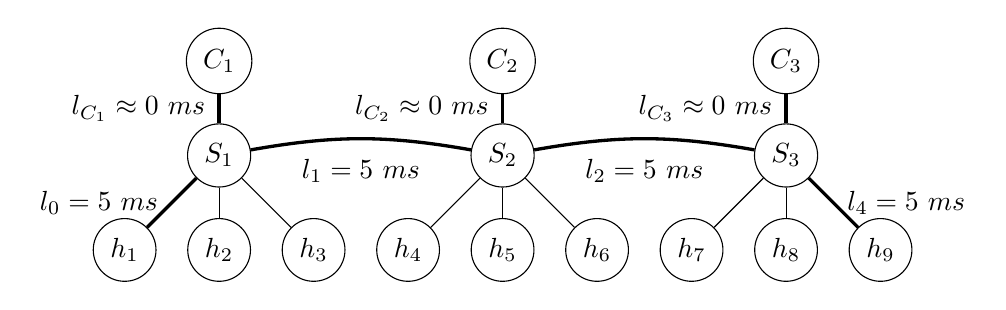
\begin{tikzpicture}[
    every node/.style={draw, circle},
    x=0.6cm,
    y=0.6cm]

    % Switches
    \foreach \n in {1,2,3} {
      \pgfmathsetmacro\x{(\n-2)*6}

      % Switch
      \node (S\n) at (\x ,  0) {$S_\n$};

      % Controller
      \node (C\n) at (\x ,  2) {$C_\n$};
      \draw (S\n) -- (C\n);

      % Hosts
      \foreach \h in {1,2,3} {
        \pgfmathsetmacro\pos{(\h - 2)*2}
        \pgfmathtruncatemacro\num{((\n - 1)*3) + int(\h)}

        % Host node
        \node (h\num) at (\x + \pos, -2) {$h_{\num}$};
        \draw (S\n) -- (h\num);
      }
    }

    % Switch links
    \draw (S1) to[out=10,in=170]
               node[below=-0.5cm, draw=none] {$l_1 = 5~ms$} (S2);

    \draw (S2) to[out=10,in=170]
               node[below=-0.5cm, draw=none] {$l_2 = 5~ms$} (S3);

    % Mark traversal path
    \draw [very thick] (h1) -- node[left,draw=none] {$l_0=5~ms$} (S1);
    \draw [very thick] (S1) -- node[left,draw=none] {$l_{C_1} \approx 0~ms$} (C1);
    \draw [very thick] (S1) to[out=10,in=170] (S2);

    \draw [very thick] (S2) -- node[left,draw=none] {$l_{C_2} \approx 0~ms$} (C2);
    \draw [very thick] (S2) to[out=10,in=170] (S3);

    \draw [very thick] (S3) -- node[left,draw=none] {$l_{C_3} \approx 0~ms$} (C3);
    \draw [very thick] (S3) -- node[right,draw=none] {$l_4=5~ms$} (h9);
  \end{tikzpicture}
  \caption{Baseline topology with three switches $S$ and their controllers
    $C$.  The client $c_0$ will send ICMP ping packets to the farthest node
      $h_9$.  The packets will go through three links with a configured
      latency of $5~ms$.}
  \label{figure:baseline.topology}
\end{figure}

Before we present the results, let's look at what we should expect from the
configuration above.  The three links the packets need to cross each have
$5~ms$ latency.  There is some latency in each switch and in each end of the
link ($c_0$ and $h_9$) as well as between and in the switches and their
controllers.

In total, one would expect the \acf{RTT} to be
\begin{gather}
  RTT_{c_0, h_9} = 2\left( \sum l + \sum P_S + \sum P_C \right) + P_{c_0} + P_{h_9} + K
  \label{equation:baseline.rtt}
\end{gather}%
that is, the latencies for all links $l$, processing time $P$ for
$S,C,c_0,h_9$ and a constant $K$ for inherent latency in the software
environment (Mininet, Open vSwitch and VirtualBox).  Equation
\ref{equation:baseline.rtt} is loosely based on
\cite{DBLP:conf/cnsm/PhemiusB13}.
\todo{Refiner formel, den kan ha feil!}

For simplicity, we will set $P_{c_0},~P_{h_9},~l_{C_1},~l_{C_2}~\text{and}~
l_{C_3}$ to zero.\footnote{When flow table entries are installed, one should
see very little traffic going to the controllers, meaning that we can
assume that $l_{C} \to 0$ after the tables are warmed up.
There are still events that are being sent from the switches to the
controllers, though.}
For consistency, we have removed the fall--back link
between $S_1$ and $S_3$ (figure \ref{figure:graph.three.switches}).
We could attempt to measure $K$ by running Mininet with two nodes linked
with zero bandwidth, but we will simply set it to zero as well.

Filling in the known values gives
\begin{gather}
  RTT_{c_0,h_9} = 40~ms + 2\left( P_S + P_C \right)
  \\
  RTT_{c_0,h_9} = 40~ms + 2L~\text{where}~L = P_S + P_C
  \label{equation:expected.baseline.rtt}
\end{gather}

We will now use the BSD \texttt{ping} command to send out packets every
$10~ms$.  The controller will install flow tables with idle and hard timeout
set to one hour.  Remember that there is some inherent noise in the system
as, e.g., ARP--packets will need to be exchanged.  The installed flow
entries will match on as many fields as possible.\todo{Cite kildekode
som vi bruker, flow installation er tatt fra POX sin l2 switch.}

On the thesis VM (for installation instructions, see chapter
\ref{chapter:install.vm}), this test can be run by opening two consoles on
and starting the POX controller first and then Mininet.

\begin{Verbatim}
# Console 1 (start first)
$ ssh mininet make bench-baseline-pox

# Console 2 (start after POX is up)
$ ssh mininet make bench-baseline-mininet
\end{Verbatim}

The results can be seen in figure
\ref{benchmark:l2.learning.switch.ping}
\vpageref{benchmark:l2.learning.switch.ping}.

We measured the \ac{RTT} and divided it by two to get an indication of the
one--way latency.\footnote{We cannot measure the \textit{true} one--way
latency, but we feel this is a good enough measure for our needs.}
\todo{Tror det er bedre å bare bruke RTT og ikke dele på to.}

An ICMP ping packet was sent every $10~ms$ with no other traffic on the
system.\footnote{Except for background noise like ARP--packets.  One can
clearly see these in the logs for the controller.}

The hard timeout for the flow table entries was set to ten seconds.  These
can clearly be seen as spikes in the plot.

\begin{figure}
  \centering
  \includegraphics[width=\textwidth]{data/pings.eps}
  \caption{Latency of ICMP ping on L2 learning switch using flow tables.}
  \label{benchmark:l2.learning.switch.ping}
\end{figure}

The median value was $16.50~ms$, the mean was $16.79~ms$.
Its \ac{RMS},

\begin{gather}
  \sqrt{\frac{1}{|n]}\sum{n^2}}
  \label{equation:rms}
\end{gather}

was $17.00~ms$.
\todo{Remove outliers and show numbers.}
The minimum and maximum values were $15.30~ms$ and $50.50~ms$.
The 1st quartile was at $16.30~ms$ and its 3rd at $16.75~ms$ and its standard
deviation $\sigma = 2.665~ms$.

\todo{Bruk boxplot() i R når en skal sammenligne. Og hiv inn tall i tabell
  for sammenligning sammen med plot. Plot trenger ikke være gigantisk stor.}

\section{L2 learning switch, key--value store}
\label{chapter:benchmark.l2.kv.noflows}

First we need a baseline.  Here we have a topology of two switches $S_0$ and
$S_1$ with a controller each.  The switches has three hosts, $h_0, \dots, h_5$.
A client $c_0$ is connected to $S_0$. We're running Python
key--value--stores on each host, and $c_0$ will issue a get--request
followed by a put--request to the host $h_5$, which is connected to $S_1$.
We measure the time for each request, divide it
by two and call it latency.\footnote{We basically assume that the packets
take an equal amount of time back and forth, and divide by two to get this
time.}

There are two controllers $C_0$ and $C_1$ for the switches $S_0$ and $S_1$,
respectively.  In this situation, the packets from $c_0$ need to travel
over two switches.

The network is running on Mininet, a software network simulator, on a Linux
virtual machine running on an Mac OS X box.  All the links in Mininet have
been set up with $10 Mbit/s$ bandwidth, $5~ms$ latency and no packet
loss.  These links have been set up with \ac{HTB}
\cite{devera2002hierarchical} enabled, which Open vSwitch\index{Open vSwitch}
 uses for providing rate limiting.

In this first benchmark, the switches will send each packet up to the
controllers.  The controllers implement L2 learning switches and will not
install any flow table entries for rapid dispatch.

On the x--axis is the time in seconds.  On the y--axis is the latency for
get and put requests.

The result can be seen in figure \ref{benchmark:l2.learning.switch.no.flows} 
\vpageref{benchmark:l2.learning.switch.no.flows}.

What is surprising here is that the put--requests have much higher latency
than the get--requests. We don't know why this is.\todo{Finn ut! Er det pga
  pakkene er større? Eller andre grunner?}

\section{L2 learning switch, key--value store, flow entries}

We have the same setup as above, but this time we install flow entries that
will automatically forward the packets.  The flow table entries will match
on as many fields in the packets as possible.

The flow table entries have idle and hard timeouts set to 10 seconds.
In other words, we should be able to see some increased latency every ten
seconds.

% Present both plots together
\begin{figure}
  \centering
  \begin{subfigure}{\textwidth}
    \centering
    \includegraphics[width=\textwidth]{data/data2.eps}
    \caption{L2 learning switch without using flow tables.}
    \label{benchmark:l2.learning.switch.no.flows}
  \end{subfigure}

  \centering
  \begin{subfigure}{\textwidth}
    \centering
    \includegraphics[width=\textwidth]{data/data3.eps}
    \caption{L2 learning switch using flow tables.}
    \label{benchmark:l2.learning.switch.with.flows}
  \end{subfigure}
\end{figure}

The result can be seen in figure \ref{benchmark:l2.learning.switch.with.flows}
\vpageref{benchmark:l2.learning.switch.with.flows}.

Here we can see that the latency has been reduced somewhat.\todo{Hvor mye?
Hva med å plotte over hverandre, hva med å lage average eller root mean
square eller noe sånn?}

We also see some latency spikes around every ten seconds, as expected.

\todo{Plott med flere verdier, istedenfor å vise seconds på x--aksen kan vi
  vise elapsed time, som i at den starter på 0 sekunder.}

These two benchmarks will serve as a baseline to which we will compare our
performance when we enable Paxos on the switches.

Remember that when we run Paxos, we will still have to use the L2 learning
switch for the nodes to be able to communicate.

\todo{Trendlinjner, moving average, fitting osv... må ha det i grafene, må
  også ha litt statistisk analyse av tallene selv osv.}

\section{Three switches, Paxos on controller}

\todo{Få data}

\section{Three switches, Paxos on controller and flow table}

\todo{Få data}

\section{Other solutions}

We chose to use OpenFlow as the basis for our system.
We could just as well have used a networking system that already supported
programmability in some way, for instance the Intel DPDK\todo{Needs
citation}.\todo{Also needs defense.}

\todo{Flytt evt dette ned til improvements--delen}

  \chapter{Improvements and future work}

Here we will discuss improvements that could have been made to our system
but was out of scope.

\section{Monitoring link--status}

OpenFlow makes it possible for controllers to receive notifications when
link status changes.  In OpenFlow 1.0, this is restricted to receiving
\textit{link up} and \textit{link down} notifications.

We could take advantage by monitoring the links to other switches.
If the leader goes down, leader--election should be performed.
If any switch goes down, then hosts should synchronize their state with
other hosts (and the same if a single host goes down).

\section{Leader--election}

Our system does not implement leader--election at all.  This should be part
of any complete Paxos system.

It would be easy to add more Paxos message types to our tables, and the
algorithms could be implemented as small bytecode programs.

\section{Using IP--fragmentation for buffering}

For the system to perform well, we don't want to store client packets in the
switch or the controller.  Instead, it would be nice if we could just pass
along client packets directly down to the end--hosts.

However, this means that the hosts will process the packets before we have a
chance to perform Paxos ordering.

We propose a neat solution to this problem.  When a switch receives a client
message, it will immediately perform IP--fragmentation of the message and
send the first fragment to the hosts.  The hosts networking stack will then
buffer the packet and wait for the last fragment.

When the Paxos consensus algorithm terminates, we will send the last
fragment down to the host, which will then pass the packet up the stack to
the server program.

We still need to store fragments, but if we choose the fragmentation offset
wisely, we need only store very small fragments.

The downside to this is that we break MTU rules, and some systems may behave
strange---or not at all.  But for our purposes we think this is a good
solution.

For this we need some new OpenFlow actions for fragmenting packets, storing
them and then forwarding the stored remaining fragment.

\section{Full Paxos support}

The most obvious improvement to this project would be to implement all of
Paxos: Trust, prepare and promise--messages and what has been mentioned
above.

However, we stated in the introduction that we wanted to constrain ourselves
to just look at how we could implement accept and learn--messages, as a
proof of concept.

Our solution would actually make it quite simple to add support for the full
Paxos algorithm.  Furthermore, our solution is very \textit{modular}, in the
sense that the controller can select which programs to compile to bytecode
and install on the switch.  This means we could have several different
leader election algorithms as small, self--contained programs, and select
which one to use for a given system.

The flow table rules are also extremely flexible as they are, and allows for
small, but easy, optimization opportunities (for instance, to support a new
Paxos message type only requires one new flow table entry and one new
program).

\todo{Flytt deler av dette ned til konklusjon, for det er et ganske sterkt
argument dette med modularisering og at det lett kan bygges videre på!}

\section{Other platforms}

Look at other programmable networks.

Openflow 2.0 is rumoured to have an experimentation api, but the stuff in
this thesis is actually far ahead of that, more flexible.
It would actually allow one to experiment with what should be part of
OpenFlow 2.0.

  \chapter{Conclusion}
\label{chapter:conclusion}

\todo{Vis at vi har nådd målene våre, vis svakheter, vis benchmark, osv. Bør
  være en ganske kort oppsummering (max en side).}



  \appendix
    \chapter{Mininet}

We've used Mininet, OpenVSwitch and POX in a VirtualBox environment to
simulate the \acp{SDN}.


    % \backmatter % <-- Only for book document class

    % Add unused citations here to make them appear in the bibliography
    % A wildcard prints out all references.
    \nocite{*}

    % These must be on ONE line without spaces
    \bibliography{bibliography/mininet,bibliography/networking,bibliography/openflow,bibliography/paxos,bibliography/sdn,bibliography/software,bibliography/source-code,bibliography/books}
    \bibliographystyle{plain}

  % Because of hyperref/makeidx/toc bug, we have to insert anchors
  % ourselves here.  See
  % http://tex.stackexchange.com/questions/138903/wrong-hyperref-for-index-in-tableofcontents-since-texlive-2010
  %
  \clearpage
  \phantomsection
  \printindex
\end{document}
